\documentclass[english,11pt]{article}

\pdfoutput=1

\usepackage[T1]{fontenc}
\usepackage[latin9]{inputenc}
\usepackage{verbatim}
\usepackage{float}
\usepackage{amsthm}
\usepackage{amsmath}
\usepackage{amssymb}
\usepackage{graphicx}
%\usepackage{multirow}
\usepackage{color}
\usepackage{url}
\usepackage{caption}
\usepackage{subcaption}
\usepackage{mathtools} 
\usepackage[margin=1.2in]{geometry}
\usepackage{showlabels}


\newcommand{\LL}{\mathcal{L}}
\newcommand{\E}{\mathbb{E}}
\newcommand{\I}{\mathcal{I}}
\newcommand{\ep}{\varepsilon}
\newcommand{\Z}{\mathbb{Z}}
\newcommand{\GCD}{\mathbf{GCD}}
\newcommand{\XX}{\mathcal{X}}
\newcommand{\SUM}{\text{sum}}
\newcommand{\1}{\mathbf{1}}
\newcommand{\rr}{\textbf{r}}
\newcommand{\ii}{\textbf{i}}
\newcommand{\jj}{\textbf{j}}

\newcommand{\II}{\mathcal{I}}
\newcommand{\kk}{\textbf{k}}
\newcommand{\RR}{\mathbb{R}}
\newcommand{\mb}{\mathbf}
\newcommand{\mk}{\mathfrak}
\newcommand{\mc}{\mathcal}

\newcommand*\Bell{\ensuremath{\boldsymbol\ell}}

\newcommand{\TODO}[1]{{\color{red}{[#1]}}}

\makeatletter

%%%%%%%%%%%%%%%%%%%%%%%%%%%%%% Textclass specific LaTeX commands.
\numberwithin{equation}{section}
%\numberwithin{figure}{section}
\theoremstyle{plain}
\newtheorem{thm}{\protect\theoremname}[section]
\theoremstyle{definition}
\newtheorem{defn}[thm]{\protect\definitionname}
\theoremstyle{remark}
\newtheorem{claim}[thm]{\protect\claimname}
\theoremstyle{plain}
\newtheorem{lem}[thm]{\protect\lemmaname}

\newtheorem*{lem*}{Lemma}

\theoremstyle{remark}
\newtheorem{rem}[thm]{\protect\remarkname}
\theoremstyle{plain}
\newtheorem{corollary}[thm]{\protect\corollaryname}
\theoremstyle{plain}
\newtheorem{proposition}[thm]{\protect\propositionname}
%%%%%%%%%%%%%%%%%%%%%%%%%%%%%% User specified LaTeX commands.
%\usepackage{slashbox}

\usepackage{babel}
\providecommand{\claimname}{Claim}
\providecommand{\definitionname}{Definition}
\providecommand{\lemmaname}{Lemma}
\providecommand{\remarkname}{Remark}
\providecommand{\theoremname}{Theorem}
\providecommand{\corollaryname}{Corollary}
\providecommand{\propositionname}{Proposition}


\newcommand{\reals}{\mathbb{R}}
\newcommand{\RL}{\mathbb{R}^L}
\newcommand{\tamir}{x}
\newcommand{\CL}{\mathbb{C}^L}
\newcommand{\RN}{\mathbb{R}^N}
\newcommand{\RNN}{\mathbb{R}^{N\times N}}
\newcommand{\RPP}{\mathbb{R}^{P\times P}}
\newcommand{\CNN}{\mathbb{C}^{N\times N}}
\newcommand{\inner}[1]{\left\langle {#1} \right\rangle}
\newcommand{\hx}{\hat{x}} 
\newcommand{\one}{\mathbf{1}} 
\newcommand{\SNR}{\ensuremath{\textsf{SNR}}}
\newcommand{\be}{\begin{equation}}
\newcommand{\ee}{\end{equation}}

\begin{document}

\title{Toward single particle reconstruction without particle picking: Breaking the detection limit}


\author{Tamir Bendory, Nicolas Boumal, William Leeb, Eitan Levin and Amit Singer}
\maketitle

\begin{abstract}
	Here comes the abstract
\end{abstract}

\section{Introduction}

\TODO{Revise--Cryo--electron microscopy (cryo--EM) is an innovative technology for single particle reconstruction (SPR) of macromolecules.} 
%In recent years, structures of many molecules, previously regarded as insurmountable, are now being reconstructed to near-atomic resolution
%; see for instance~\cite{kuhlbrandt2014resolution,bartesaghi20152,smith2014beyond}.
%This technological advancement was recognized by the 2017 Nobel Prize in Chemistry~\cite{nobel}. 
% 
In a cryo--EM experiment, biological samples are rapidly frozen in a thin layer of vitreous ice. Within the ice, the molecules are randomly oriented and positioned. The microscope produces a 2-D tomographic image of the samples embedded in the ice, called a \emph{micrograph}. Each micrograph contains tomographic projections of the samples at unknown locations and under unknown viewing directions. The goal is to construct 3-D models of the molecules from the micrographs.

The signal to noise ratio ($\SNR$) of the projections in the micrographs is a function of two dominating factors. On the one hand, the $\SNR$ is a function of the electron dose. To keep radiation damage within acceptable bounds, the dose must be kept low, which leads to high noise levels. On the other hand, the $\SNR$ is a function of the molecule \TODO{size/weight}. The smaller the molecules, the fewer detected electrons carry information about them.

%\paragraph{Particle picking.}
All contemporary methods in the field split the reconstruction procedure into several stages.
The first stage consists in extracting the various particle projections from the micrographs. This stage is called \emph{particle picking}. Later stages aim to construct a 3-D model of the molecule from these projections. The quality of the reconstruction eventually hinges on the quality of the particle picking stage. Figure~\ref{fig:micro_example} illustrates how particle picking becomes increasingly challenging as the $\SNR$ degrades.

Crucially, it can be shown that reliable detection of individual particles is impossible below a certain critical $\SNR$; see for instance~\cite{bendory2018estimation}\TODO{To verify the title}. This fact has been recognized early on by the cryo-EM community. In particular, in an influential paper from 1995, Henderson~\cite{henderson1995limitations} investigates the following questions:
\begin{quote}
	\emph{For the purposes of this review, I would like to ask the question: what is the smallest size of free-standing molecule whose structure can in principle be determined by phase-contrast electron microscopy? Given what has already been demonstrated in published work, this reduces to the question: what is the smallest size of molecule for which it is possible to determine from images of unstained molecules the five parameters needed to define accurately its orientation (three parameters) and position (two parameters) so that averaging can be performed?}
\end{quote}
In that paper and in others that followed (e.g.,~\cite{glaeser1999electron}), it was established that particle picking is impossible for molecules below a certain weight (below $\sim$50 kDa). 
Joachim Frank voices a similar observation in his Nobel prize lecture: ``\emph{Using the ribosome as an example, it became clear from the formula we obtained that the single-particle approach to structure research was indeed feasible for molecules of sufficient size: Particle Size > 3/[Contrast$^2\times $  Resolution (as length) $\times$ Critical Electron Dose]}''~\cite{frank2018single}. 
\TODO{As these two leaders of the cryo-EM community point out,} it is impossible to reconstruct small molecules by any of the existing computational pipelines for single particle analysis in cryo--EM, because the particles themselves cannot be picked from the micrographs.

The unique issues raised by small particles have been mitigated by recent technological advances in the field, including the use of Volta phase plates~\cite{khoshouei2017cryo,liang2017phase} and scaffolding cages~\cite{liu2018nearatomic}.
%
Despite this progress, detecting small molecules in the micrographs remains a challenge.
We note that nuclear magnetic resonance (NMR) spectroscopy and X-ray crystallography are well suited to reconstruct small molecules. Yet, cryo--EM has a lot to offer even for molecules with already known structures obtained via NMR spectroscopy or X-ray crystallography, because these methods have limited ability to distinguish conformational variability. \TODO{Need a ref for this claim.}

In this paper, we argue that there is a gap between the two questions in Henderson's quoted excerpt above, and that one may be able to exploit it to design better reconstruction algorithms.
Specifically, the impossibility of particle picking does not necessarily imply impossibility of particle reconstruction.
Indeed, the aim is only to reconstruct the molecule: estimating the locations of the particles in the micrograph is merely a helpful intermediate stage when it can be done. Our main message is that the limits particle picking imposes on molecule size do not translate into limits on particle reconstruction.

As a proof of concept, we study a simplified model for 3-D reconstruction directly from the micrograph on a simulated data. 
In order to recover the 3-D volume, we use autocorrelation analysis. In a nutshell, we relate the autocorrelations of the micrographs to the autocorrelations of the volume.
For any noise level, these autocorrelations can be estimated to any desired accuracy, provided the we get to observe sufficiently many particle projections and the latter are separated in the micrograph. Importantly, there is no need to detect the projections. The autocorrelations of the micrographs are straightforward to compute and require only one pass over the data. These directly yield estimates for the autocorrelations of the volume. To estimate the volume itself from its estimated autocorrelations, we solve a nonlinear inverse problem via least-squares. In this controlled experiment, we make several simplified assumptions; see the Discussion Section for details. 
As a side note, we mention that expectation-maximization (EM)---a popular framework in SPR---is intractable for this problem; see~\cite{bendory2018estimation} for the details. \TODO{Do we want to stress that we get only low-resolution of the volume?}


Another interesting feature of the described approach pertains to model bias, whose importance in cryo-EM was stressed by a number of authors~\cite{shatsky2009method,vanheel1992correlation,henderson2013avoiding,vanheel2013finding}. In the classical ``Einstein from noise'' experiment, multiple realizations of pure noise are aligned to a picture of Einstein using template matching and then averaged. In~\cite{shatsky2009method}, it was shown that the averaged noise rapidly becomes remarkably similar to the Einstein template. In the context of cryo--EM, this experiment exemplifies how prior assumptions about the particles may influence the reconstructed structure. This model bias is common to all particle picking methods based on template matching. In our approach, no templates are required, thus significantly reducing concerns about model bias. \TODO{To add reference to our example.}


% while neglecting important aspects as discussed in detail in TKTK. 

%In first model, an unknown image appears numerous times at unknown locations in several micrographs, each affected by additive Gaussian noise---see Figure~\ref{fig:micro_example} for an illustration.
%The goal is to estimate the planted image. The task is interesting in particular when the $\SNR$ is low enough that particle picking cannot be done reliably. This problem is interesting of its own as it appears in other scientific applications, such as spike sorting~\cite{lewicki1998review}, passive radar~\cite{gogineni2017passive} and system identification~\cite{ljung1998system}. We study it in more details in a companion paper~\cite{bendory2018estimation}. An extension to multiple planted images is analyzed in~\cite{bendory2018estimation}.
%
%In the second model, we consider the 3-D reconstruction problem as it appears in cryo-EM, \TODO{Here we need to elaborate a bit.} This is the main result of this paper. \TODO{We probably need to switch the order of this paragraph.}

%A precise mathematical formulation of the model, including an extension where more than one planted images are to be recovered, is provided in Section~\ref{sec:methods}.
%To be clear, we do not consider here many prominent features of real SPR experiments and do not aim to reconstruct any 3-D structure. Instead, we solve a simpler problem that we believe captures key elements of the SPR problem. We note that similar models emerge in spike sorting~\cite{lewicki1998review}, passive radar~\cite{gogineni2017passive} and system identification~\cite{ljung1998system}.

%In order to recover the 3-D volume, we use autocorrelation analysis. In a nutshell, we relate the autocorrelation functions of the micrographs to the autocorrelation functions of the volume.
%For any noise level, these autocorrelations can be estimated to any desired accuracy, provided the projections are well separated and we acquire enough of them. Importantly, there is no need to detect the projections. The autocorrelations of the micrographs are straightforward to compute and require only one pass over the data. These directly yield estimates for the autocorrelations of the volume. To estimate the volume itself from its estimated autocorrelations, we solve a nonlinear inverse problem via least-squares. 
%We use similar technique for the simpler model of planted image as illustrated in Figure~\ref{fig:Einst_example}. 

To illustrate the possibility to estimate a signal without detecting its locations, we first discuss a toy model for which it is easier to convey the mathematical principles. 
In this toy model, an unknown image appears numerous times at unknown locations in several micrographs, each affected by additive Gaussian noise---see Figure~TKTK for an illustration.
The goal is to estimate the planted image. The task is interesting in particular when the $\SNR$ is low enough that particle picking cannot be done reliably. 
This problem is interesting of its own as it appears in other scientific applications, such as spike sorting~\cite{lewicki1998review}, passive radar~\cite{gogineni2017passive} and system identification~\cite{ljung1998system}. We study it in more details, including an extension to multiple planted images, in a companion paper~\cite{bendory2018estimation}.

%




\begin{figure}[t]
	\centering
	\begin{subfigure}[h]{0.33\textwidth}
		\centering
		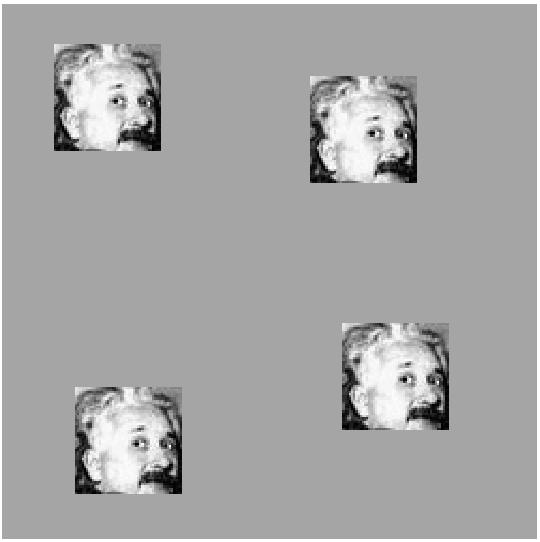
\includegraphics[scale=0.5]{micrograph_Einstein_example_clean}
		\caption{$\sigma = 0$}
	\end{subfigure}%
	\begin{subfigure}[h]{0.33\textwidth}
		\centering
		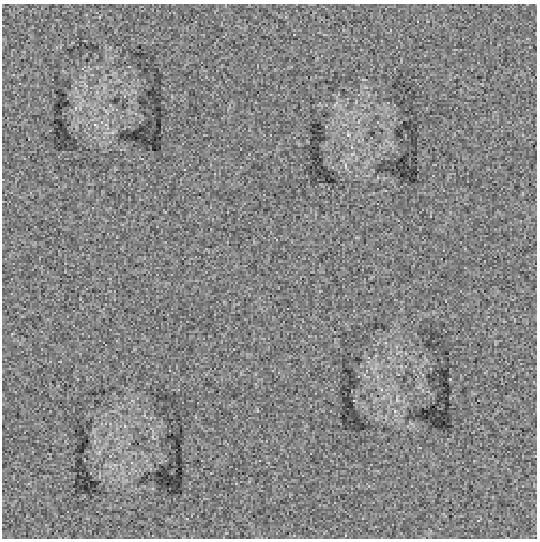
\includegraphics[scale=0.5]{micrograph_Einstein_example_s05}
		\caption{$\sigma = 0.5$}
	\end{subfigure}
	\begin{subfigure}[h]{0.33\textwidth}
		\centering
		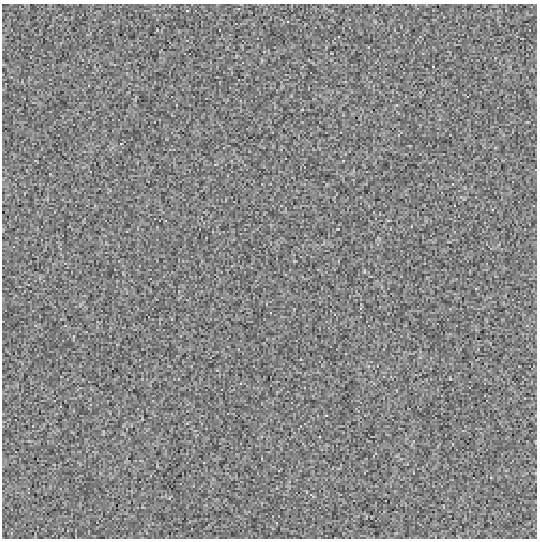
\includegraphics[scale=0.5]{micrograph_Einstein_example_s3}
		\caption{$\sigma = 3$}
	\end{subfigure}
	\caption{\label{fig:micro_example} Example of micrographs of size $250\times 250$ with additive white Gaussian noise of variance $\sigma^2$ for increasing values of $\sigma$. Each micrograph contains the same four occurrences of a $50 \times 50$ image of Einstein. In panel (c), the noise level is such that it is very challenging to locate the occurrences of the planted image. In fact, it can be shown that at low $\SNR$, reliable detection of individual image occurrences is impossible, even if the true image is known. By analogy to cryo-EM, this depicts a scenario where particle picking cannot be done. \TODO{Do we want to replace with a cryo-EM figure?}}	
\end{figure}


\section{Results} \label{sec:results}

The techniques we advocate allow to recover a signal hidden in noisy micrographs without (even implicitly) detecting the location of signal repetitions in these micrographs. To illustrate the underlying principles of the method, it is instructive to start with a toy model where the target signal is an unknown 2-D image. The latter appears several times in noisy micrographs, at unknown locations. Toward recovery, we first compute the second-order autocorrelation of the micrographs. We then establish that the autocorrelation of the target image can be recovered from the autocorrelation of the micrographs in a straightforward manner. The more micrographs we collect, the more accurate the estimate of the image's autocorrelation. 
The target image is then estimated from its autocorrelation using a standard inversion algorithm (up to elementary symmetries).
The same principles carry over to the more challenging task of 3-D reconstruction from micrographs.
The Methods Section provides additional details. 

In the  experiment, we estimated Einstein's image of size $50\times 50$ and mean zero from a growing number of micrographs, each of size $4096\times 4096$ pixels. A micrograph contains, on average, 700 occurrences of the target image at random locations. 
Thus, about 10\% of each micrograph contains signal. The micrographs are contaminated with additive white Gaussian noise with standard deviation $\sigma=3$ (this corresponds to $\SNR=1/20$). This high noise level is illustrated in TKTK. %In this first experiment, we assume knowledge of $\sigma$ and of the total number of signal occurrences across all micrographs.\TODO{Need to mention that in the 3-D reconstruction we do not make these assumptions.}
To simplify the experiment, we assume the number of signal occurrences and the noise standard deviation are known. Micrographs are generated such that any two occurrences are always separated by at least 49 pixels in each direction. The separation restriction is discussed in more details in the Methods Section.

We compute the average second-order autocorrelation of the micrographs. This is a particularly simple computation which can be efficiently executed with a fast Fourier transform (FFT) on GPUs. In the Methods Section, we show how, owing to separation of the occurrences, a determined portion of the averaged autocorrelation allows to estimate the autocorrelation of the unknown image itself. Mathematically, it can be shown that for any noise level, the quality of this estimate improves steadily as the amount of data grows~\cite{bendory2018estimation}. Then, to estimate the target image, we resort to a standard phase retrieval algorithm called relaxed-reflect-reflect (RRR)~\cite{elser2017rrr}, initialized randomly.

%RRR is initialized far away from the ground truth, and it iterates to produce the estimate, up to a reflection ambiguity.

Figure~\ref{fig:Einst_example} shows several estimated images for a growing number of micrographs, and a movie is available in \TODO{supplementary material}. Figure~\ref{fig:error_per_micro} presents the normalized recovery error as a function of the amount of data available. Error is measured as the ratio of the root mean square error (RMSE) to the norm of the ground truth (square root of the sum of squared pixel intensities.) This is computed after fixing elementary symmetries (see Methods.) As evidenced by these figures, the ground truth image can be estimated increasingly well from increasingly many micrographs, without particle picking.
\TODO{Tamir: I will rewrite it with the new experiment.}
\TODO{Here the cryo-EM setup shows up}

%defined as 
%\begin{equation}
%\text{RMSE}  := \frac{\|x - \hat{x}\|_{\text{F}}}{\|x \|_{\text{F}}},
%\end{equation} 
%where $x$ and $\hat{x}$ are, respectively, the underlying and estimated image, and $\|\cdot\|_{\text{F}}$ stands for the Frobenius norm.  
%\TODO{We have a movie in the supplementary material.}

%%%% This is about bias, and it's imprecise; let's leave it out?
%As an initial guess, we picked an image of the physicist Issac Newton. If the algorithm was prone to model bias, we would expect to get as an output an image that resembles Newton, similarly to the ``Einstein from noise.'' However, the experiment exhibits the desired phenomenon: the more data we collect, the better the reconstruction quality. 



\begin{figure}[h!]
	\centering
	\begin{subfigure}[h]{0.45\textwidth}
		\centering
		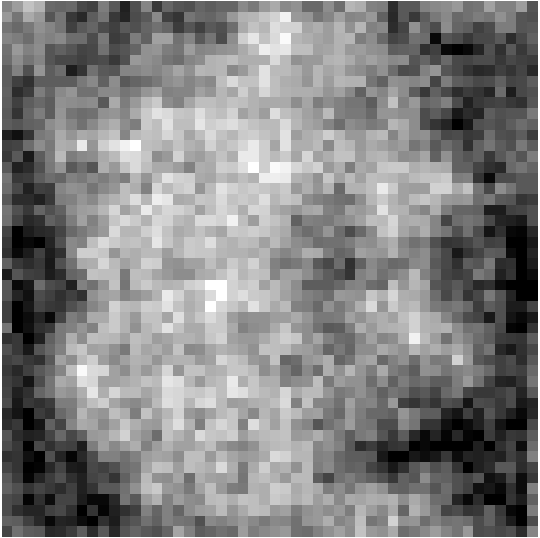
\includegraphics[scale=0.45]{reconstruction1_cropped}
		\caption{\small $P = 512$}
	\end{subfigure}%
	\begin{subfigure}[h]{0.45\textwidth}
		\centering
		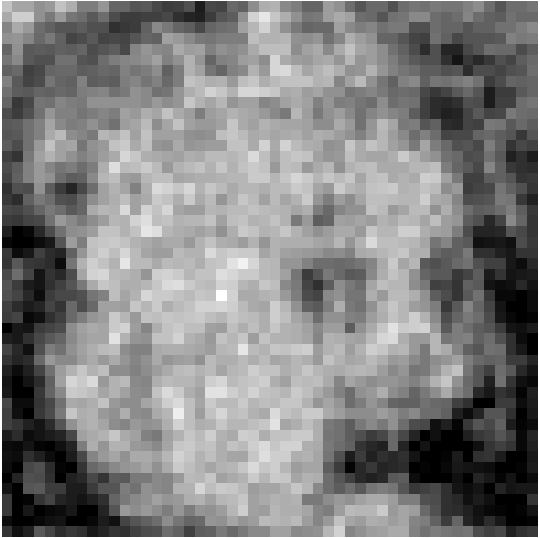
\includegraphics[scale=0.45]{reconstruction10_cropped}
		\caption{\small $P = 512\times 10$}
	\end{subfigure}%

		\begin{subfigure}[h]{0.45\textwidth}
		\centering
		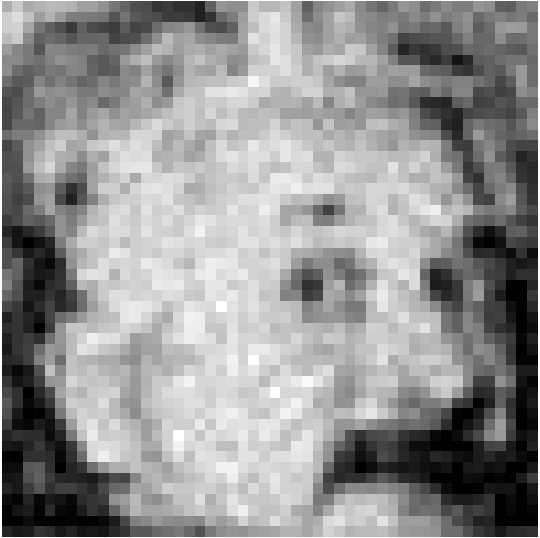
\includegraphics[scale=0.45]{reconstruction100_cropped}
		\caption{ \small $P = 512\times 10^2$ }
	\end{subfigure}%
	\begin{subfigure}[h]{0.45\textwidth}
		\centering
		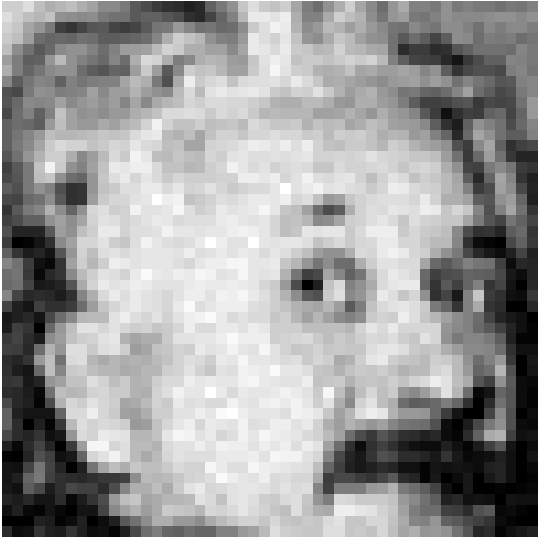
\includegraphics[scale=0.45]{reconstruction1000_cropped}
		\caption{\small $P = 512\times 10^3$}
	\end{subfigure}%

%	\begin{subfigure}[h]{0.33\textwidth}
%		\centering
%		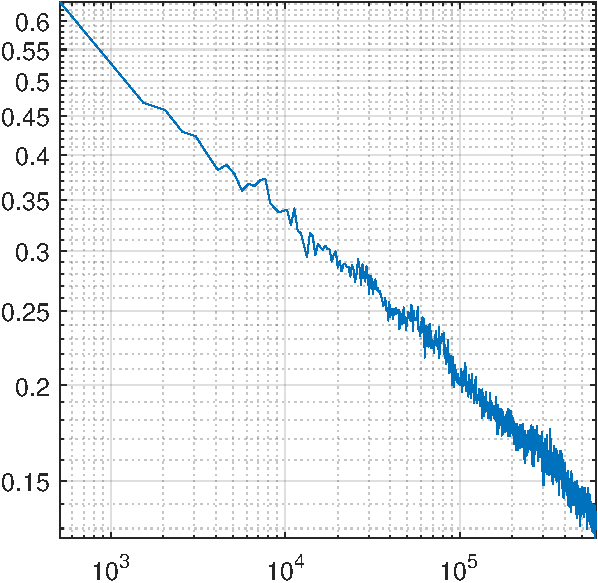
\includegraphics[scale=0.33]{Einstein_progress_cropped}
%		\caption{\label{fig:err_curve}\small Error curve}
%	\end{subfigure}%

%\begin{figure}[h!]
%	\centering
%	\begin{subfigure}[h]{0.25\textwidth}
%		\centering
%		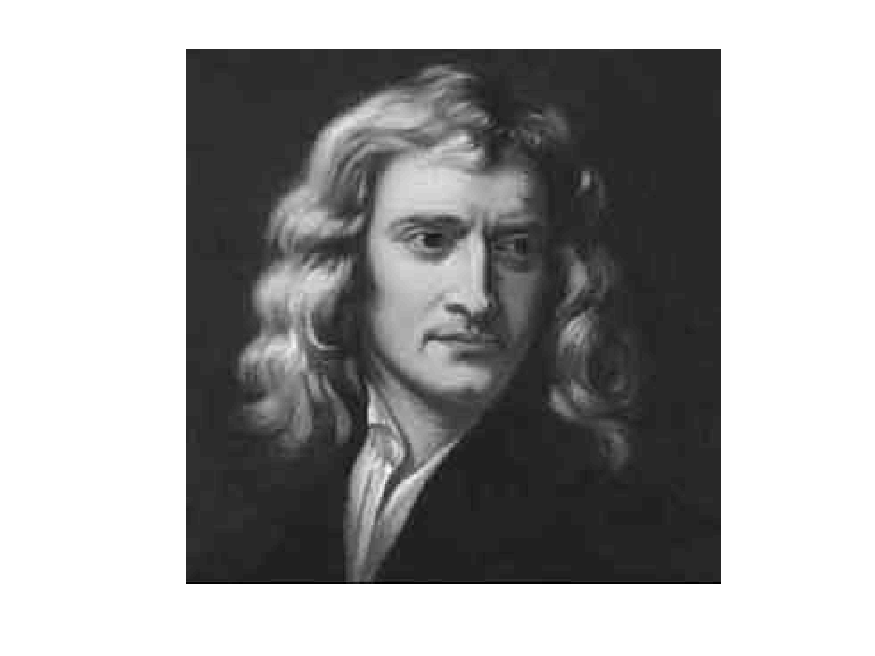
\includegraphics[scale=0.3]{Newton}
%		\caption{\label{fig:newton}Newton  (model)}
%	\end{subfigure}%
%	\begin{subfigure}[h]{0.25\textwidth}
%		\centering
%		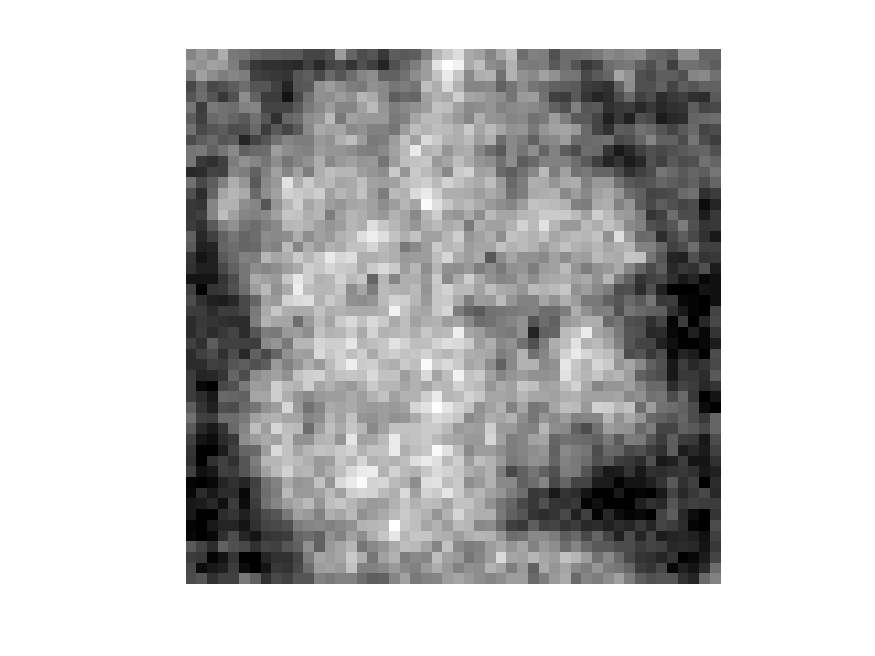
\includegraphics[scale=0.3]{reconstruction2}
%		\caption{\small $P =1024$}
%	\end{subfigure}%
%	\begin{subfigure}[h]{0.25\textwidth}
%		\centering
%		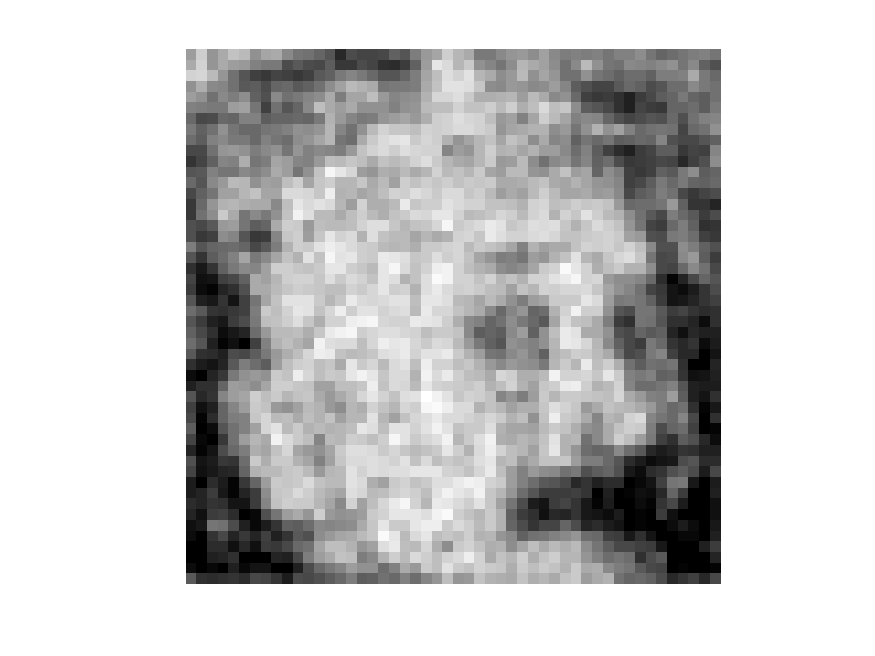
\includegraphics[scale=0.3]{reconstruction20}
%		\caption{$P = 1024\times 10$}
%	\end{subfigure}%
%	\begin{subfigure}[h]{0.25\textwidth}
%		\centering
%		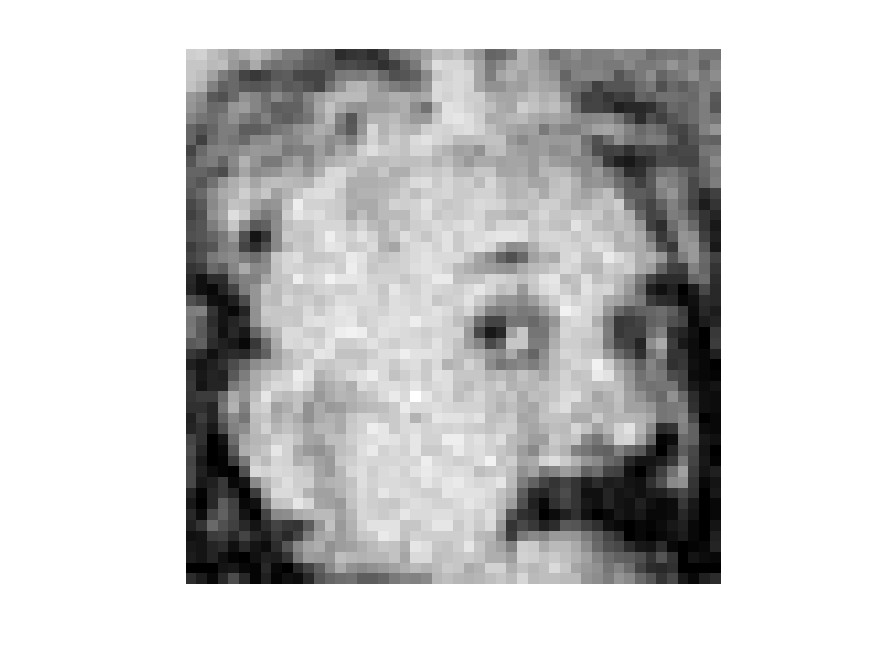
\includegraphics[scale=0.3]{reconstruction200}
%		\caption{$P = 1024\times 100$}
%	\end{subfigure}%
	\caption{\label{fig:Einst_example} Recovery of Einstein from micrographs at noise level $\sigma = 3$ (see Figure~\ref{fig:micro_example}(c)). Averaged autocorrelations of the micrographs allow to estimate the power spectrum of the target image. This does not require particle picking. A phase retrieval algorithm (RRR) produces the estimates here shown, initialized with an image of the physicist Isaac Newton. Estimates are obtained from $P$ micrographs (growing across panels), each containing $700$ image occurrences on average.
		\TODO{To add: redo the figures according to Amit's comments and the figures of noisy Einstein's micrographs}
		% At a noise level of $\sigma = 3$, this amounts to an $\SNR$ of $1/20$.
	}
\end{figure}



\begin{figure}[h]
\centering
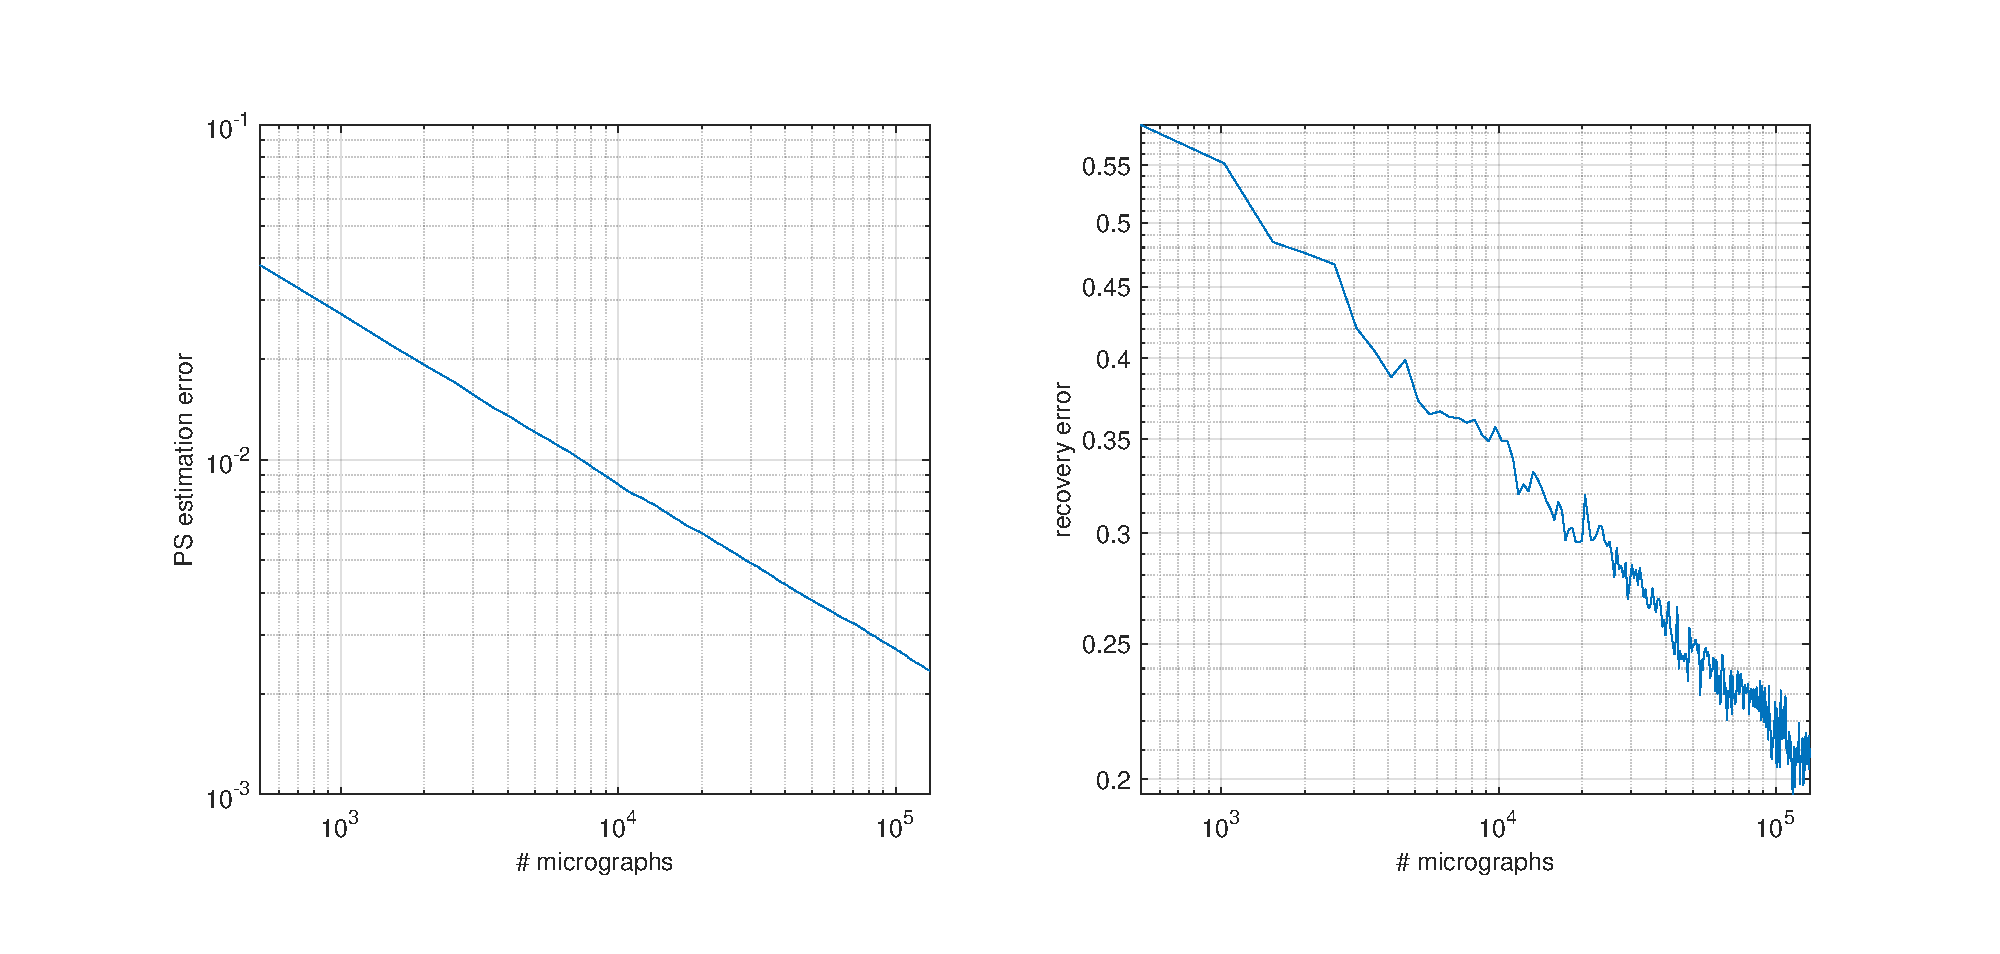
\includegraphics[scale=.7]{Einstein_progress}
\caption{\label{fig:error_per_micro} Relative root mean square error of the estimate of Einstein's image as a function of the number of observed micrographs (logarithmic scale along both axes.)}
\end{figure}



%
%Figure~\ref{fig:1Dheterosignals} demonstrates accurate estimation of three signals simultaneously with noise level $\sigma=3$. We define the ratio of the space occupied by the $i$th signal as 
%\begin{equation}
%\gamma_i = \frac{M_i L}{N},
%\end{equation}
%where $M_i$ is the signal's number of occurrences, $L$ is the length of the signal and $N$ is the micrograph length. In the experiment, we do not assume to know these ratios, neither the noise level $\sigma$. As can be seen, given enough signals occurrences, we can estimate accurately the signals. he estimation quality 
%is poorer than the other two signals, a phenomenon that can be explained using Proposition~\ref{prop:uniqueness}.

%
%In the second experiment, three 1-D signals, each of length $L = 21$, appear at random locations in one long 1-D signal, which we call a micrograph by analogy. Any two occurrences are separated by at least 20 entries. The signals appear respectively about 30, 20 and 10 million times in a micrograph of length 12.3 billion. The micrograph is then contaminated with additive white Gaussian noise. This results in an $\SNR$ of about $1/9$, while about 10\% of the micrograph contains signal. Neither the number of occurrences nor the noise level $\sigma$ are known to the algorithm.
%
%In the Methods section, we detail how autocorrelations of the micrograph can be used to estimate weighted averages of the autocorrelations of the target signals. The individual signals and their relative densities are then estimated from autocorrelations up to order three by solving a nonlinear least-squares problem.
%
%Figure~\ref{fig:1Dheterosignals} shows how the estimates improve as we see a larger and larger fraction of the micrograph (that is, as more and more data becomes available.) As is clear from the picture, despite the high noise level which would make it very challenging to locate the individual signal occurrences, the signals can be estimated accurately given enough data. Furthermore, the \TODO{propensity\footnote{Might not be the right word; 'density' is not good because it might refer to the density of the particle for example, whereas here we mean to say the 'fraction of occurrences that come from a particular class'}} of each signal can also be estimated.

%In order to estimate the signals, we computed the first three autocorrelation functions of the data and then estimated the signals and their corresponding $\gamma_i$ using a nonconvex least-squares. 
%As can be seen, given enough signal occurrences, we can estimate accurately the signals. 
%The estimation quality of the triangle signal is poorer than the other two signals, a phenomenon that is explained using Proposition~\ref{prop:uniqueness}.

%We do not assume the knowledge of the noise level. 
%Crucially, starting from the point of $n\approx10^8$, the RMSE of the signal estimation decreases linearly with slope $-1/2$---the expected estimation rate of the autocorrelation functions---implying the stability of the recovery algorithm. 
%
%\begin{figure}[t]
%	\centering
%	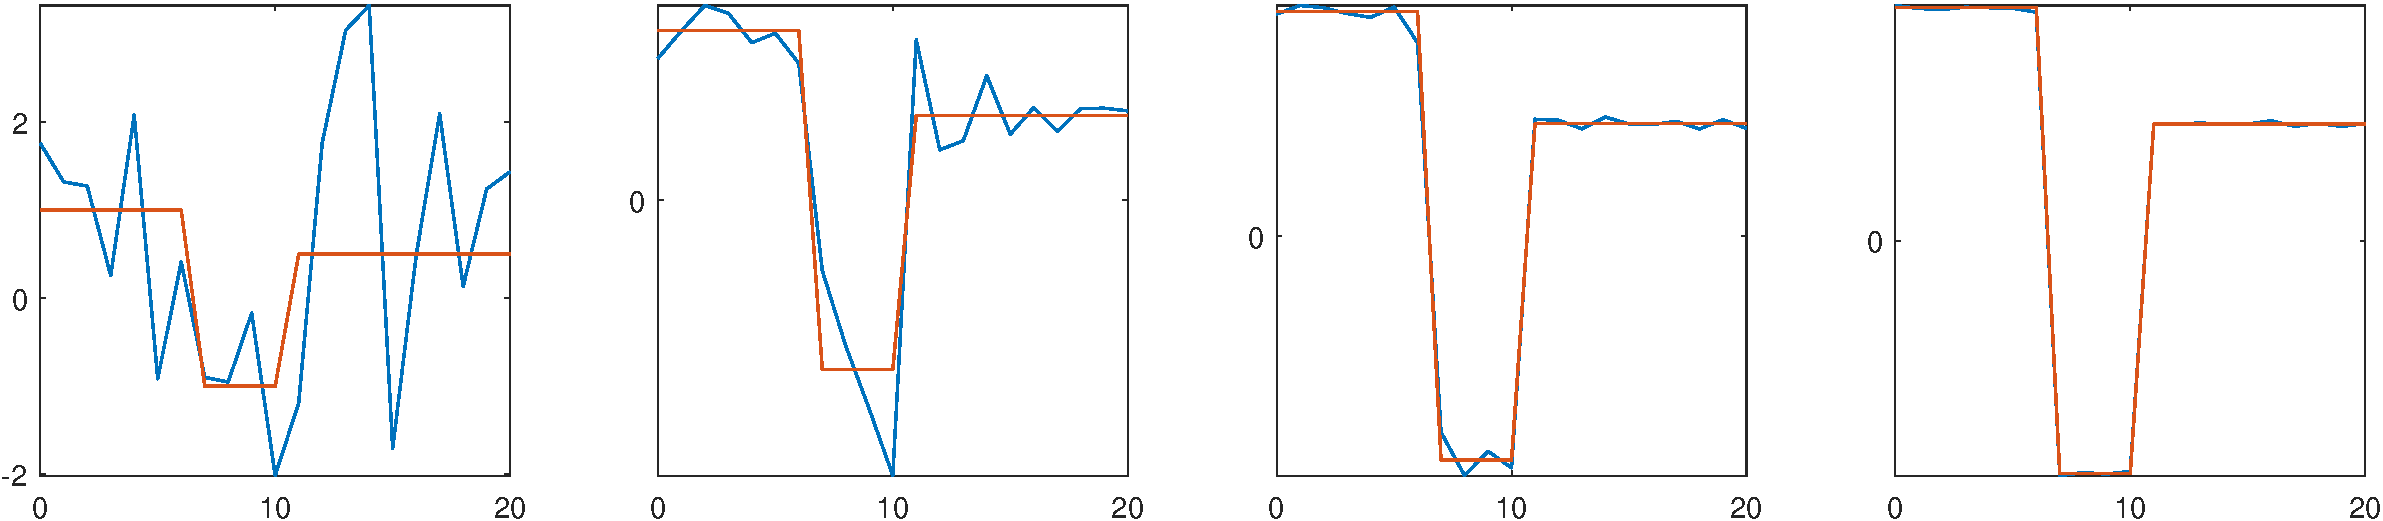
\includegraphics[scale=0.45]{progressive_n}
%	\caption{\TODO{...} \TODO{This figure is with new ROI method based on loss functions}}
%	\label{fig:1Dhomosignals}
%\end{figure}
%
%\begin{figure}[t]
%	\centering
%	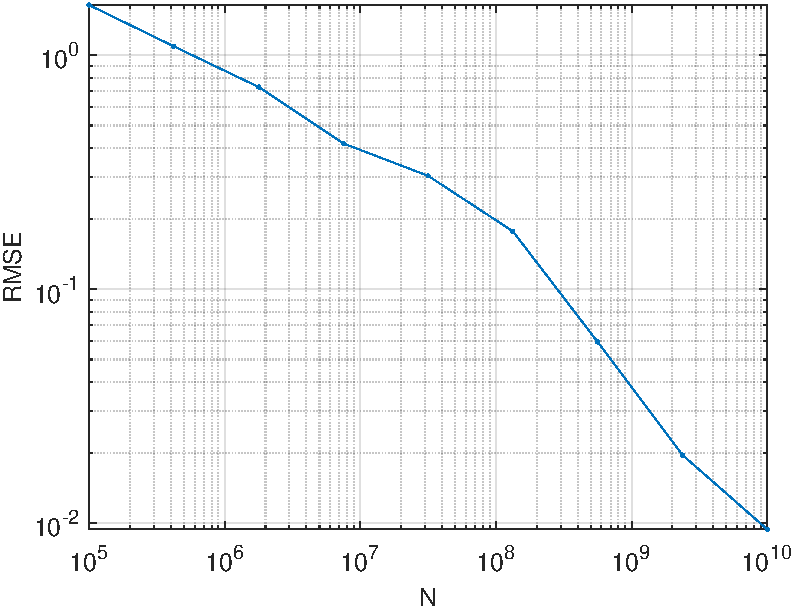
\includegraphics[width=0.5\linewidth]{XP_1D_homogeneous_new_ROI/progressive_RMSE_n}
%	\caption{\TODO{...} \TODO{This figure is with new ROI method based on loss functions}}
%	\label{fig:1DhomoRMSE}
%\end{figure}

%
%\begin{figure}[t]
%	\centering
%	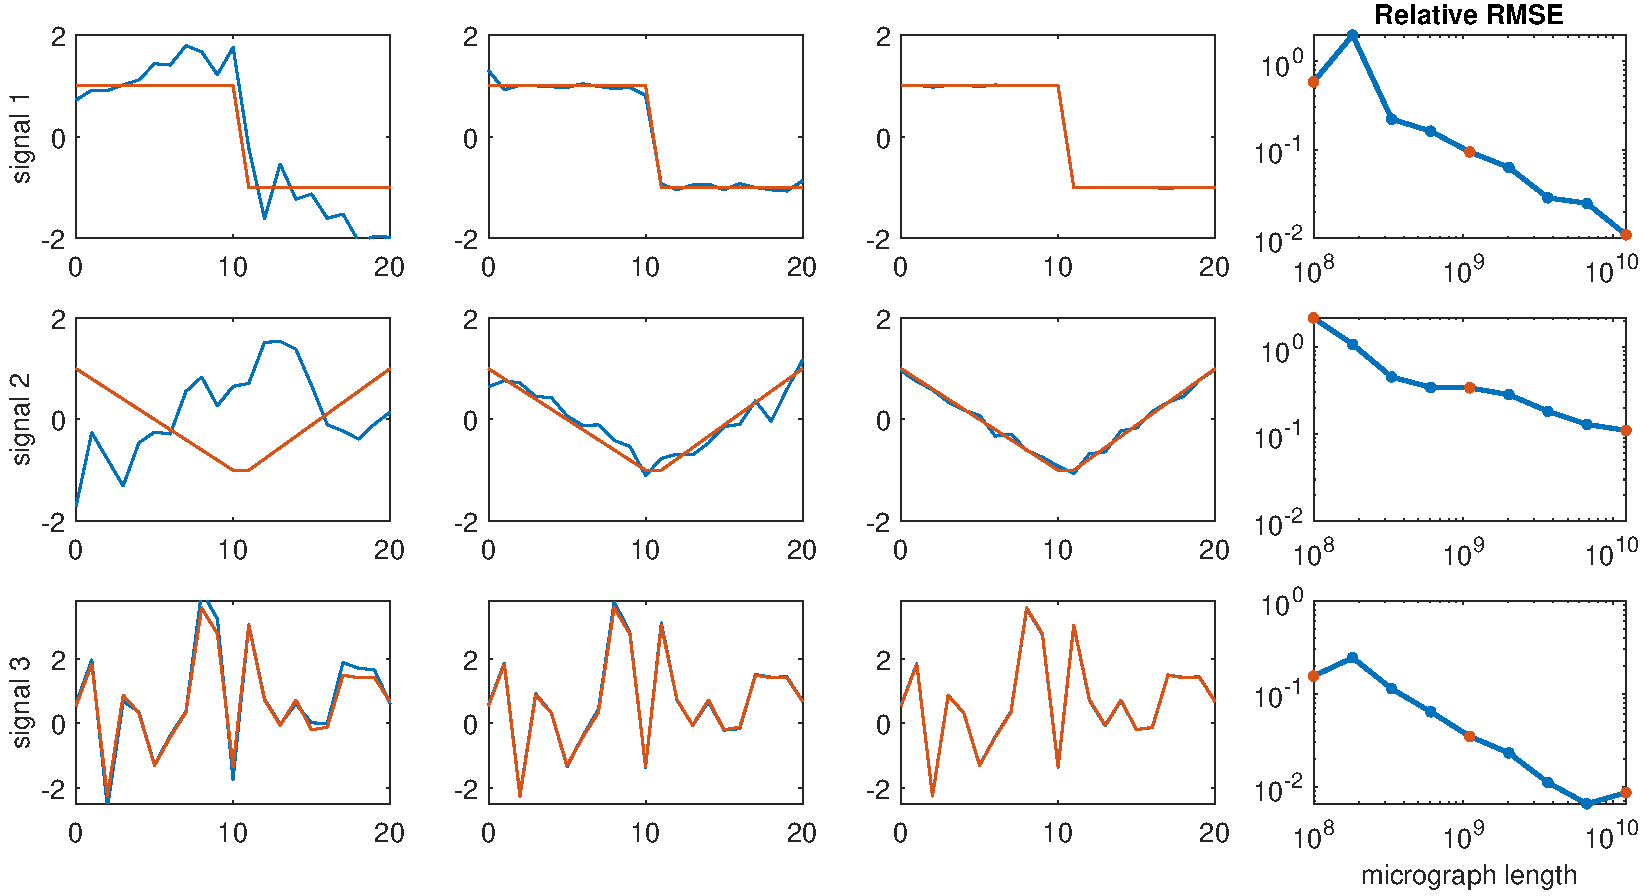
\includegraphics[width=\linewidth]{heterogeneous_progressive_n12300000000_466300}
%	\caption{For the second experiment, each row shows, three times, one of the target signals (red), overlaid with an estimate (blue) obtained from a growing portion of the noisy micrograph (about $10^8$, $10^9$ and $10^{10}$ entries available to compute autocorrelations). The last column depicts evolution of the relative root mean square error in estimating each individual target signal. Signals 1 to 3 appear respectively about 30.0, 20.0 and 10.0 million times. With the whole micrograph available, the algorithm estimated those to be 29.8, 21.9 and 10.0 million, respectively.
%%		
%%		An experiment for estimate three one-dimensional signals simultaneously with noise level $\sigma=3$. Red signals are the ground truth (targets) and the blue signals are our estimations. Individual RMSE of the estimates: $0.0239393 / 0.208925 / 0.0335956$. The estimated $\gamma$'s are $0.02574 / 0.01693 / 0.00818$ and the true ones $0.02561 / 0.01707 / 0.00853$. The $\SNR$ is $1/12$. \TODO{1. to replace with a ``progress'' plot 2. replace the triangle signal 3. add error progress figure}
%	}
%	\label{fig:1Dheterosignals}
%\end{figure}



\clearpage
\section{Discussion}


In the simplified model for cryo-EM we examined, we showed it is possible to estimate the 3-D structure of small volumes. 
Our strategy is to compute autocorrelation functions of the micrographs and to relate these statistics to the unknown volume's parameters. Recovering the parameters from the statistics reduces to solving a set of polynomial equations.
Crucially, the outlined approach involves no particle picking, hence a fortiori no viewing direction estimation. Concerns for model bias are also greatly reduced since no template matching is involved.

Looking towards applying the framework to encompass all important features of real cryo-EM experiments, our work implies that it might be possible to reconstruct small molecules, in particular, molecules that are too small to be detected in micrographs. 
In pursuing this research direction, our goal is to significantly increase the range of molecules to which cryo-EM can be successfully applied.
We recognize that significant challenges lay ahead for the implementation of the proposed approach to 3-D reconstruction directly from the micrographs. We discuss a few now.


%As a result, it may not be limited to large molecules in the same way that particle picking approaches are. 
%In this paper, we illustrated that it is possible to determine the 3-D molecular structure in single particle cryo-EM directly from the micrographs without performing particle picking, at least in controlled experiments. 


\TODO{
	We should also incorporate Alberto's comment that our technique also allows to use much lower defocus values. Lower defocus means lower contrast, but will maintain higher frequency information. From that perspective, we may be able to get high resolution reconstructions from fewer micrographs, just because we would be using lower defocus. }

%All current algorithmic pipelines for SPR using cryo--EM start with a particle picking algorithm which is prone to model bias. 
%Bypassing the particle picking stage and constructing a 3-D model directly from the data---without assuming prior knowledge on the particle to be estimated---can be used to reconstruct ab initio models to initialize a refinement algorithm.  Alternatively, it can be applied to generate templates for a particle picker which does not suffer from model bias.


%In the simplified model we examined, the aim is to estimate one, or possibly several, images from micrographs. Our strategy is to compute autocorrelation functions of the data and to relate these statistics to the unknown parameters. Recovering the parameters from the statistics reduces to solving a set of polynomial equations. Depending on the scenario, we did so using either a phase retrieval algorithm or a nonlinear least-squares algorithm.
%


 %Depending on the scenario, we did so using either a phase retrieval algorithm or a nonlinear least-squares algorithm.

%
%The same general approach can, in principle, be applied directly to SPR from cryo-EM. Here, the micrographs contain numerous tomographic projections of molecules (possibly in different conformations) taken from unknown viewing directions. The aim is to estimate the 3-D volumes of the different conformations directly from micrographs. Each volume can be expanded linearly in a basis, so that the volume is characterized by its expansion coefficients. Since tomographic projection is a linear operation, autocorrelations of the micrographs (which can be estimated easily) are polynomial functions of the sought coefficients. Thus, autocorrelations of the micrographs provide a system of polynomial equations in the volume parameters, and the question becomes: are these equations sufficient to uniquely identify the volumes, and can we solve the system?
%
%We show in Appendix~\ref{sec:cryoem} that the number of polynomial equations provided by the third-order autocorrelations is of the same order as the number of coefficients required to describe one volume \TODO{at resolution comparable to that of the particle projections---remove?}. This hints that it may be possible to reconstruct one or even several distinct volumes from these equations directly. Additional parameters in these equations could encode an unknown viewing direction distribution and an unknown conformation distribution, which could then also be estimated. Crucially, the outlined approach involves no particle picking, hence a fortiori no viewing direction estimation or conformation clustering. As a result, it may not be limited to large molecules in the same way that particle picking approaches are. Concerns for model bias would also greatly be reduced.


%While the field is currently dominated by Bayesian methods such as EM, they are intractable for such problems. As an alternative, we propose to use autocorrelation analysis technique that shares some common lines (did you get the wordplay?)  with Kam's method for ab initio modeling~\cite{kam1980reconstruction,levin20173d,singer2018mathematics}. That being said, the SPR model is far more complicated than the model presented here. In a future research, we hope to bridge this gap.

One possible concern is that the numerical experiments conducted here suggest a large amount of data may be necessary.\footnote{Whether or not this large amount of data would be necessary for any method to succeed given the unfavorable $\SNR$ is an interesting research question.} Recent trends in high-throughput cryo-EM technology \TODO{?} give hope that this may be a lesser concern in the long term. Still, large amounts of data also imply large amounts of computations. On this front, we note that computing autocorrelations can be executed efficiently on CPUs and GPUs, and in parallel across micrographs. It can even be done in streaming mode, as only one look at each micrograph is necessary. The output of this data processing stage is a succinct summary in the form of autocorrelation estimates: its size is a function of the resolution, not a function of the number of observed micrographs. Subsequent steps, which involve solving the system of polynomial equations, scale only in the size of that summary. Of course, an important question then is whether the equations can be solved meaningfully in practice. The proof-of-concept experiments above suggest they might.

%Insofar as the computational challenges are concerned, we note that expectation-maximization algorithms (EM) have, over time, become the norm in the cryo-EM community, as exemplified by the popular RELION package. The idea of using EM for cryo-EM can be traced back at least to~\TODO{Sigworth}. At the time, such approaches also seemed challenging.


%\TODO{Do we want to say something about the number of images that we need? Specifically, do we want to address the fact that the numerical experiments suggest we may need a gigantic number of them for cryo, and mention trends in cryo technology that are encouraging in that regard? (Of course, we can't compare to RELION etc.\ in SNRs so low that one can't particle pick; that's not the point here.)}

Beyond data acquisition and computational challenges, there are modeling issues to consider.
As stated, our approach relies on two core assumptions that are not necessarily verified in SPR experiments.
First, we assume an additive white noise model, while in practice the noise may be correlated or signal dependent. To address this point, it may be necessary to investigate better noise models and to incorporate power spectrum estimation methods. % and to extend the autocorrelation analysis accordingly. 
 Second, we assume that any two particles are sufficiently separated, and we use this assumption to derive algebraic relations between autocorrelations of the micrographs and autocorrelations of the 3-D volume. 
Perhaps this separation could be induced by careful experimental design \TODO{?}.
Alternatively, if the signals are not well separated, one can introduce new parameters which encode the distribution of the spacing between occurrences. Here as well, relations between autocorrelations of the micrographs and of the volume could be derived.

We also note several aspects of SPR experiments that were neglected in this paper, including Contrast Transfer Function (CTF) correction and the non-uniformity of the viewing directions. All these aspects must be taken into account so the method could be applied on real data. We hope to take care of these issues in future research, as well to extend the proposed method to conformational heterogeneity. 
\TODO{another issue is that micrographs also contain contaminants such as carbon, ice crystals, etc.. }
%
%\TODO{Do we want to note here that EM used to be perceived as computationally out of reach back when it was proposed [cite Fred], yet is now the de facto standard method as exemplified by RELION? Do we also want to stress that models have been refined over decades? Both points are rather defensive in nature.	}

\TODO{Where and how do we cite Kam? Fred?}

\section{Methods} \label{sec:methods}

\subsection{Toy 2-D experiment}

Let $x\in\RPP$ be the target image and let $y\in\RNN$ be  one of  $K$ observed micrographs. 
%If more than one micrograph is available, then it is sufficient to average the autocorrelations we compute below over the micrographs.
Independently for each micrograph, the image formation model is as follows. An unknown binary signal $s\in\{0,1\}^{(N-P)\times(N-P)}$ indicates the starting positions of all occurrences of $x$ in $y$, so that, with additive white Gaussian noise, we observe:
\begin{align}
	y & =  x \ast s + \varepsilon, & \varepsilon & \sim \mathcal{N}(0,\sigma^2I),
	\label{eq:model}
\end{align}
where $\ast$ denotes linear convolution, $\ii:=(i_1,i_2)$ identifies one location in the image and $\ii=(0,0)$ indicates the  upper left corner.
We define the images to be zero outside their support.
The binary signals $s$ obey the following separation property: 
\begin{align}
	\textrm{If } s[\ii] = 1 \textrm{, then } s[\jj] = 0  \textrm{   for all $\jj=(j_1,j_2)$ such that   }  \max\{\vert i_1-j_1\vert, \vert i_2-j_2\vert\}\leq 2P-1.
	\label{eq:spacing}
\end{align}
In words: the upper left corners of any two occurrences of the target image $x$ in a micrograph must be separated by at least $2P-1$ pixels in each direction.
Hence, each image is separated by a signal-free area that will ease the interpretation of the autocorrelation analysis. 
From the micrographs, we aim to  recover $x$ only. In this simplified model, we assume  the total number of  occurrences of the signal across micrographs is known. 
In the 3-D experiment we do not assume knowledge of the number of projections in the micrographs.
%In contrast, particle picking is the task of estimating the binary signal $s $, which cannot  be performed reliably if $\sigma$ is large (that is, at low $\SNR$.)


%
%\section{Autocorrelation analysis}   \label{sec:autocorrelation}
%
%Our method for estimating the signals is composed of two stages. 
%First, we use the autocorrelation functions of the data to estimate a mixture (i.e., linear combination) of the $K$ signal's autocorrelations. The mixed autocorrelation can be estimated to any accuracy, in any $\SNR$ level, if $M$ is large enough and the spacing condition~\eqref{eq:spacing} is met. Then, we  use a nonconvex LS  to estimate the signals from their mixed autocorrelations. 
%In this section, we elaborate on the autocorrelation functions and their estimations, while the precise recovery procedure, based on nonconvex optimization, will be discussed in detail in the next section.

%\paragraph{Aperiodic autocorrelation functions.}
The second-order autocorrelation of  an arbitrary image $z\in\mathbb{R}^{m\times m}$ is defined by
  \begin{align} 
 a_z^2[\Bell] & = \frac{1}{N^2} \sum_{i_1 = \max\{0, -\ell_1\}}^{m-1 + \min\{0, -\ell_1\}} \sum_{i_2 = \max\{0, -\ell_2\}}^{m-1 + \min\{0, -\ell_2\}}z[\ii]z[\ii+\Bell]. 
 \end{align}
 Below, the image $z$ might be either a target image $x$ or the micrograph $y$. 
 It can be shown that in the limit of infinitely many micrographs $K\to\infty$,  the mean pixel value of the micrographs is equal to the mean pixel value of the signal $x$, scaled by  
 \begin{align} \label{eq:gamma}
 \gamma & = \frac{M P^2}{N^2},
 \end{align}
 where $M$ is the number of occurrences of $x$ across micrographs. 
 This  is the fraction of entries of all micrographs occupied by occurrences of $x$, that is, the  density of the signal. 
  The spacing constraint~\eqref{eq:spacing} imposes $\gamma\leq\frac{P}{2P-1}\approx 1/2$.


 % Similarly, as $K\to\infty$ the second-order autocorrelations are related through 
 Similarly, numbering micrographs as $y_1, \ldots, y_K$, the empirical average of the second-order autocorrelations of the micrographs converges as follows:
 \begin{align} \label{eq:a2}
	\lim_{K \to \infty} \frac{1}{K} \sum_{k=1}^{K} a_{y_k}^2[\Bell] & = \gamma a_{x}^2[\Bell] + \sigma^2\delta_{(0,0)}[\Bell], \quad \Bell\in[0,P-1]^2,
 \end{align}
 where $\delta_{(i,j)}[\Bell]=1$ for $\Bell=(i,j)$ and zero otherwise.
 Thus, for any noise level and without the need to even implicitly locate the images $x$ in the micrographs, given sufficiently many micrographs we are able to compute the second-order autocorrelation of $x$ itself. Recovering $x$ from $a_x^2$ can be done up to symmetries, as detailed below.
 Equation~\eqref{eq:a2} is proven and its extension to higher-order autocorrelations and multiple distinct planted images is discussed in~\cite{bendory2018estimation}. 


%\paragraph{Numerical experiment with a 2-D image.}

For the 2-D experiment shown in Figures~\ref{fig:Einst_example} and~\ref{fig:error_per_micro}, we generate $K$ micrographs of size $4096\times 4096$ pixels. 
In each micrograph, we place Einstein's image (of zero mean) of size $50\times 50$  in random locations, while preserving the separation condition~\eqref{eq:spacing}.  
This is done by randomly selecting $4000$ placements in the micrograph, one at a time with
an accept/reject rule based on the separation constraint and locations picked so far.
On average, $700$ images are placed in each micrograph.   
Then, i.i.d.\ Gaussian noise with standard deviation $\sigma=3$ is added, inducing an $\SNR$ of approximately $1/20$.
An example of a micrograph's excerpt is presented in the right panel of Figure~TKTK.
%Different micrographs are handled sequentially on a GPU, as GPUs are particularly well suited to execute simple instructions across large vectors of data. If multiple GPUs are available, segments can of course be handled in parallel.


In this experiment, we assume $\gamma$ and the noise level $\sigma$ are known. In this setup, the second-order autocorrelation determines almost any target image uniquely, up to reflection through the origin~\cite{hayes1982reconstruction}. The second-order autocorrelation can be computed at the cost of one 2-D FFT per micrograph. These can be computed highly efficiently and in parallel. To recover the image $x$ itself, we use a standard algorithm used for phase retrieval called relaxed-reflect-reflect (RRR)~\cite{elser2017rrr}.

%
%To recover the target image from the estimated power spectrum, we use a standard phase retrieval algorithm called relaxed-reflect-reflect (RRR). This algorithm iterates the map
%\begin{align*}
%	z & \leftarrow z + \beta (P_2(2P_1(z) - z) - P_1(z))
%\end{align*}
%on an image $z$ of size $2L\times 2L$.
%We set the parameter $\beta$ to 1.
%The map is designed so that, if the estimated power spectrum is exact, then fixed points contain Einstein's image in the upper-left corner of size $L \times L$, possibly reflected through its origin, and zeros elsewhere. The operator $P_2(z)$ combines the Fourier phases of  the current estimation $z$ with the estimated Fourier magnitudes. The operator $P_1(z)$ zeros out all entries of $z$ outside the $L\times L$ upper-left corner. 

In order to compare the performance in multiple cases and at different noise levels, the RRR is stopped after a fixed number of iterations (1000)\TODO{check} and the iterate with the smallest error compared to the ground truth (up to the reflection ambiguity) is chosen as the solution. 
While this cannot be done in practice (since we do not have access to the ground truth to determine which iterate is best), this procedure enables us to compare a large number of instances in different noise environments. \TODO{Note the last two sentences!}
\TODO{Let's try with the last iterate and see}

\subsection{3-D experiment}

Let $\phi$ be the Coulomb potential representing the molecule we aim to recover. 
We assume that molecule is real-valued and smooth. In spherical coordinates, its 3-D Fourier transform $\widehat\phi$ admits a finite expansion of the form
\be\label{eq:volume_expansion} 
\widehat \phi(k, \theta, \varphi) = \sum_{\ell = 0}^L\sum_{m=-\ell}^{\ell}\sum_{s=1}^{S(\ell)}\tamir_{\ell, m, s}Y_{\ell}^m(\theta,\varphi)j_{\ell,s}(k),
\ee
where $Y_{\ell}^m$ are complex spherical harmonics and $j_{\ell,s}$ are normalized spherical Bessel functions; see Appendix TKTK for further definitions.  Let $I_{\omega}$ denote the tomographic projection obtained from viewing direction $\omega\in SO(3)$. By the Fourier projection-slice theorem, its 2-D Fourier transform  is given by~\cite{natterer1986mathematics}:
\be\label{eq:projection_model}
\widehat I_{\omega}(k,\varphi) = \sum_{\ell,m,m',s}\tamir_{\ell,m,s}D_{m',m}^{\ell}(\omega)Y_{\ell}^{m'}\left(\frac{\pi}{2},\varphi\right)j_{\ell,s}(k),\ee
where $D_{m',m}^{\ell}(\omega)$ is a Wigner-D matrix.

Let $\II\in\RNN$ denote a micrograph. We assume it consists of shifted copies of projections contaminated by additive white Gaussian noise:
\begin{equation}\label{eq:micrograph_model}
\II = \sum_{t=1}^{M} I_{\omega_t}\ast\delta_{\mb s_t}+ \varepsilon, \quad \varepsilon~\sim\mathcal{N}(0,\sigma^2 I),
\end{equation}
where the viewing directions $\omega_t$ are assumed to be drawn from the uniform distribution over $\text{SO}(3)$ and $\mb s_t$ denotes the location of the center of the $t$th projection in the micrograph. Similarly to~\eqref{eq:spacing}, we impose a separation condition so that any two projections are separated by at least $2P-1$ pixels between their upper left corners  in each direction.
%similarly to~\eqref{eq:spacing}:
%\be\label{eq:sep_cond} \ ||\mb s_j - \mb s_i||_{\infty} \geq 2L. \ee
Note that~\eqref{eq:model} can be also written as a sum of $\delta$ functions as in~\eqref{eq:micrograph_model}. 
%\TODO{Say something about nonuniformity in practice? Remember that biologists will jump at this...}

Define the $p$th autocorrelation of $\II$ as
\begin{equation*} \label{eq:Kth_autocorrelation}
a^p_\II(\Bell_1,\ldots, \Bell_{p-1}) = \frac{1}{N^2}\sum_{\mb i}\II[\Bell]\II([\mb i+\Bell]_1)\cdots \II([\mb i+\Bell]_{p-1}),
\end{equation*}
where the summation is for $\mb i $ ranging over the $N^2$  pixels of the micrograph. %, $\Bell = (\Delta i, \Delta j)$.% and we set $\II(i,j)=0$ if either $i,j\notin\{1,\ldots, M\}$. 
%In our procedure, we compute the first three autocorrelations. %, called the mean, power spectrum, and bispectrum, of the micrographs. \TODO{This definition and terminology should come earlier}. 
Let $\II_1,\ldots\II_K$ denote a set of $K$ micrographs. 
Under the specified conditions, we show in Appendix~\ref{sec:moment_derivation} that the first three autocorrelations  of the micrographs are related to those of the projections by \begin{align} \label{eq:ac_micrographs}
\lim_{K\to\infty}\frac{1}{K}\sum_{i=1}^Ka^p_{\II_i}[\Bell_1,\ldots,\Bell_{p-1}]  &= \gamma\left\langle a^p_{I_\omega}[\Bell_1,\ldots,\Bell_{p-1}]\right\rangle_{\omega} + b_p[\Bell_1,\ldots,\Bell_{p-1}], \\ p=1,2,3,& \quad \Bell_1,\ldots,\Bell_{p-1}\in[-(P-1),P-1]^2, \nonumber
\end{align}
where $\langle\cdot\rangle_\omega$ denotes averaging over all possible viewing directions $\omega$ and $b_p$ is a bias term. %and we take the limit as the number of projections $N$, and hence the dimensions of the micrograph $M$, tend to $\infty$. 
Specifically,  $b_1 = 0$ and therefore the mean is unbiased. The bias term of the second-order autocorrelation  $b_2$ depends only on $\sigma^2$, the variance of the noise. Hence, if the noise level can be accurately estimated from the micrographs, this bias can be removed. 
Finally, the bias term of the third-order autocorrelation $b_3$ depends on the mean of the micrograph and $\sigma^2$.  Therefore, given sufficiently many projections, we can accurately estimate the quantities $\gamma\langle a^p_{I_{\omega}}\rangle_{\omega}$ directly from the micrographs. These quantities are functions of the unknown coefficients $\tamir_{l,m,s}$ and we could proceed to invert their relation, as we did in the 2-D toy example. 

In practice, we want to leverage one more feature of the 3-D reconstruction problem.
Since all in-plane rotations of the micrographs are equally likely observations, 
it is desirable in~\eqref{eq:ac_micrographs} to average over all in-plane rotations as well.
This can be done efficiently using Prolate Spheroidal Wave Functions (PSWFs).  We use autocorrelations up to and including the  third order since this is necessary to  determine the volume.
The details are in the appendix. 

% as follows. We scan the micrographs with a $P\times P$ window. We expand each window in Prolate Spheroidal Wave Functions (PSWFs) 
%and compute the  second and third autocorrelations in that basis. In PSWFs, it is straightforward to average over all in-plane rotations~\cite{landa2017steerable,zhao2016fast}. We further average over all windows, resulting in autocorrelation in the PSWF coefficients.
%It can be shown that the PSWF coefficients of the data $\mathfrak{a}^p$  are related to the expansion coefficients of the volume~\eqref{eq:volume_expansion} by
%\begin{align}\label{eq:coeffs_to_moms}
%&\mathfrak{a}^1_x = \frac{L}{\sqrt{4\pi}}\sum_sa_{0,0,s}j_{0,s}(0), \\ 
%&\mathfrak{a}^2_x(q) = \frac{1}{2\sqrt{2\pi}}\sum_{\substack{\ell,m\\s_1,s_2}}C_2^{(q)}(\ell,s_1,s_2)a_{\ell,m,s_1}\overline{a_{\ell,m,s_2}},
% \\
%&\mathfrak{a}^3_x(k,q_1,q_2) = \sum_{\substack{\ell_1,m_1,s_1\\\ell_2,m_2,s_2\\s_3}}\sum_{\ell_3=|\ell_1-\ell_2|}^{\min(L,\ell_1+\ell_2)}C_3^{(k,q_1,q_2)}(\ell_1,m_1,s_1;\ell_2,m_2,s_2;\ell_3,s_3)a_{\ell_1,m_1,s_1}a_{\ell_2,m_2,s_2}\overline{a_{\ell_3,m_1+m_2,s_3}}.
%\end{align}
%The definitions of $C_2$ and $C_3$ are provided in Appendix TKTK.
%
%To recover the expansion coefficients $\{a_{\ell,m,s}\}$ from the autocorrelation coefficients estimated from the micrograph $\mk m_k[\II]$, we minimize the weighted least-squares problem
%\be\label{eq:min_problem_cryo} \min_{\{a_{\ell,m,s}\}} \sum_{k=1}^3\frac{\Big|\Big|\mk m_k\{a_{\ell,m,s}\} - \mk m_k[\II]\Big|\Big|_F^2}{||\mk m_k[\II]||_F^2}.\ee

\section*{Acknowledgment}
Let's thank them all

\bibliographystyle{plain}
\bibliography{ref}



\appendix


\section{Moments derivation} \label{sec:moment_derivation}
In this section we prove relation~\eqref{eq:ac_micrographs}. We note that mathematically taking infinitely many micrographs is equivalent to take one infinitely large micrograph with fixed density $\gamma$~\eqref{eq:gamma}. Hence, we consider the moments of one micrograph $\II$ in the limit $N\to\infty$ and  $\gamma = \lim_{N\to\infty}\frac{MP^2}{N^2}\in(0,1)$. %To take this limit, we shall assume that $N=\Omega(M^2)$, and that $\gamma = \lim_{N\to\infty}\frac{NL^2}{M^2}\in(0,1)$ is a constant. 
The separation condition guarantees that if $\mb i=(i,j)$ is in the support of some projection, then $\mb i + \mb \Bell$ for $\Bell\in[-(P-1),P-1]^2$ is either in the support of the same projection or outside the support of any projection. %Formally, $\mb i$ is in the support of the $j$th projection if and only if $0\leq \mb i - \mb s_j < L$ where the inequalities apply to each coordinate. Then for $||\Bell||_{\infty}\leq L-1$ we have
%\[-(L-1) \leq [\mb i+\Bell]-\mb s_j< 2L-1,\]
%and because of the separation condition, given $\mb s_k$ we must either have $\mb s_k-\mb s_i\geq 2L-1$ in which case 
%\[ \mb i + \Bell- \mb s_k \leq \mb i + \Bell- \mb s_j - (2L-1) < 0,\]
%or $\mb s_k - \mb s_i \leq -(2L-1)$, in which case
%\[ \mb i + \Bell - \mb s_k \geq -(L-1) + 2L-1 = L.\]
%In either case, $[\mb i+\Bell]$ is not in the support of the $k$th particle.

We begin by calculating the relation between the $p$th autocorrelation of the clean micrograph and the  averaged autocorrelation of the projections.
Let us denote the clean micrograph by $\widetilde \II = \II-\varepsilon$, where $\II$ and $\varepsilon$ are given in~\eqref{eq:micrograph_model}.     
Denote by $\mc S_t$ the support of the $t$th particle. % and by $Z=\{1,\ldots, M\}-\sqcup_j \mc S_j$ all the points outside the support of the particle. %The clean  micrograph  then satisfies $\widetilde \II[\Bell] = 0$ if $\mb i\in Z$, so we have
 Then, we have
\be\begin{aligned} \label{eq:general_moment}
a^p_{\widetilde\II}[\Bell_1,\ldots, \Bell_{p-1}] &= \frac{1}{N^2}\sum_{\mb i}\widetilde\II[\mb i]\widetilde\II[\mb i + \Bell_1]\cdots \widetilde\II[\mb i + \Bell_{p-1}]\\
&= \frac{1}{N^2}\sum_{t=1}^M\sum_{\mb i\in\mc S_t}\widetilde\II[\mb i]\widetilde\II[\mb i + \Bell_1]\cdots \widetilde\II[\mb i + \Bell_{p-1}] \\ %+ \frac{1}{N^2}\sum_{\mb i\in Z}\widetilde\II[\Bell]\widetilde\II[\mb i + \Bell]\cdots \widetilde\II(\mb i + \Bell_{p-1})\\
&= \frac{MP^2}{N^2}\cdot\frac{1}{M}\sum_{t=1}^M\frac{1}{P^2}\sum_{i,j=0}^{P-1} I_{\omega_t}[\mb i]I_{\omega_t}[\mb i+\Bell_1]\cdots I_{\omega_t}[\mb i + \Bell_{p-1}]\\
&= \frac{MP^2}{N^2}\frac{1}{M}\sum_{t=1}^Ma^p_{I_{\omega_t}}[\Bell_1,\ldots, \Bell_{p-1}]\\
&\to \gamma\langle a^p_{I_{\omega}}[\Bell_1,\ldots, \Bell_{p-1}]\rangle_{\omega}, \end{aligned}\ee
where the average is taken over $\omega$ with respect to the distribution of viewing directions. Here, we assume it to be uniform.


In the presence of noise, we get additional bias terms denoted by $b_p$ in~\eqref{eq:ac_micrographs}. The mean ($p=1$) is unbiased  since the noise is assumed to have zero mean. For the second-order autocorrelation ($p=2$), we have
\[\begin{aligned} 
a^2_\II[\Bell] &=
\frac{1}{N^2}\sum_{\mb i }\II[\mb i]\II[\mb
i+\Bell]\\
&= \frac{1}{N^2}\sum_{\mb i }\widetilde\II[\mb i]\widetilde\II[\mb i+\Bell] + \frac{1}{N^2}\sum_{\mb i }\widetilde\II[\mb i]\varepsilon[\mb i + \Bell]\\ &+ \frac{1}{N^2}\sum_{\mb i }\varepsilon[\mb i]\widetilde\II[\mb i + \Bell] + \frac{1}{N^2}\sum_{\mb i }\varepsilon[\mb i]\varepsilon[\mb i + \Bell]. 
\end{aligned}\]
The first term is given by~\eqref{eq:general_moment} for $p=2$. 
The cross terms vanish in the limit. 
%Considering the terms one-by-one, the first term is independent of the
%noise, and as shown above converges to $\gamma \langle
%m_2[I_{\omega}]\rangle_{\omega}$ as $N\to\infty$. The second term
%satisfies
%\[\begin{aligned} 
%\frac{1}{N^2}\sum_{\mb i}\widetilde\II[\Bell]\varepsilon[\mb i + \Bell] &=
%\frac{NL^2}{M^2}\cdot\frac{1}{NL^2}\sum_{j, \mb i}I_{\omega_j}(\mb
%i)\varepsilon_{\omega_j}[\mb i + \Bell]\\
%&\to \gamma\mathbb{E}_{\omega,\varepsilon}[I_{\omega}\varepsilon]\\ 
%&= \gamma \mathbb{E}_{\omega}[I_{\omega}]\mathbb{E}_{\varepsilon}[\varepsilon] = 0, \end{aligned}\]
%where $\varepsilon_{\omega_j}[\Bell] = \varepsilon(\mb i + \mb s_j)$ and we used the fact that the orientations $\omega$ and the noise $\varepsilon$ are independent, and $\mathbb{E}_{\omega}[I_{\omega}] = \langle m_1[I_{\omega}]\rangle_{\omega}$. A similar argument applied to the third term shows that it
%also vanishes as $N\to\infty$. 
The fourth term is zero unless $\Bell=0$, in which case it converges to $\sigma^2$.
% $\Bell \neq \mb{0}$ %then since the noise is zero mean and
%i.i.d. this term vanishes. If $\Bell = \mb0$ then
%\[ \frac{1}{N^2}\sum_{i,j=1}^m\varepsilon[\Bell]^2 \to \sigma^2.\]
Thus, we conclude
\[ a^2_\II[\Bell] \to \gamma\langle a^2_{I_{\omega}}[\Bell]\rangle_{\omega} + \sigma^2\delta[\Bell],\]
where the  bias term $b_2[\Bell] = \sigma^2\delta[\Bell]$   depends only on the variance of the noise $\sigma^2$.


For the third moments, we get 8 terms:
\[\begin{aligned} 
&a^3_\II[\Bell_1, \Bell_2] =
\underbrace{\frac{1}{N^2}\sum_{\mb i}\widetilde\II[\mb i]\widetilde\II[\mb i+\Bell_1]\widetilde\II[\mb i + \Bell_2]}_{(1)} +
\underbrace{\frac{1}{N^2}\sum_{\mb i}\varepsilon[\mb i]\varepsilon[\mb i+\Bell_1]\varepsilon[\mb i + \Bell_2]}_{(2)}\\ 
&+ \underbrace{\frac{1}{N^2}\sum_{\mb i}\widetilde\II[\mb i]\varepsilon[\mb i + \Bell_1]\widetilde\II[\mb i + \Bell_2]}_{(3)} +
\underbrace{\frac{1}{N^2}\sum_{\mb i}\widetilde\II[\mb i]\widetilde\II[\mb i + \Bell_1]\varepsilon[\mb i + \Bell_2]}_{(4)}\\
&+ \underbrace{\frac{1}{N^2}\sum_{\mb i}\varepsilon[\mb i]\widetilde\II[\mb i + \Bell_1]\widetilde\II[\mb i + \Bell_2]}_{(5)} +
\underbrace{\frac{1}{N^2}\sum_{\mb i}\widetilde\II[\mb i]\varepsilon[\mb i + \Bell_1]\varepsilon[\mb i + \Bell_2]}_{(6)}\\
&+ \underbrace{\frac{1}{N^2}\sum_{\mb i}\varepsilon[\mb i]\varepsilon[\mb i + \Bell_1]\widetilde\II[\mb i + \Bell_2]}_{(7)} +
\underbrace{\frac{1}{N^2}\sum_{\mb i}\varepsilon[\mb i]\widetilde\II[\mb i + \Bell_1]\varepsilon[\mb i + \Bell_2]}_{(8)}.
\end{aligned}\]
We address these terms one by one:
\begin{itemize}
	\item  Term (1) is treated by~\eqref{eq:general_moment} for $p=3$;
	\item Term (2) is the third-order autocorrelation of  pure noise  which vanishes in the limit; 
	\item Terms (3)-(5) depend linearly on the noise and hence
	vanish in the limit;
	\item For term (6), if $\Bell_1\neq \Bell_2$ the term
	vanishes in the limit. If $\Bell_1 = \Bell_2$ then
	\[ \begin{aligned}
        \frac{1}{N^2}\sum_{\mb i}\widetilde\II[\mb i]\varepsilon[\mb i + \Bell]^2
      &= \frac{MP^2}{N^2}\cdot\frac{1}{MP^2}\sum_{t=1}^{M}\sum_{\mb i\in\mc S_t}I_{\omega_t}[\mb i]\varepsilon[\mb i + \Bell]^2 
      \to \gamma\sigma^2 \langle a^1_{I_{\omega}}\rangle_{\omega}, %\gamma\mathbb{E}_{\omega, \varepsilon}[\varepsilon^2I_{\omga}]\\
      %&= \gamma\sigma^2\mathbb{E}[m_1[I_{\omega}]]\\ 
      %&= \gamma\sigma^2Lm_1[\phi],
    \end{aligned}\]
	where $\langle a^1_{I_{\omega}}\rangle_{\omega}$ is the mean of the volume. 
	\item  Terms (7) and (8) contribute $\delta$ functions similar to (6).
	%That is because by the Fourier projection-slice theorem, the Fourier transform of the projections correspond to the restriction of the 3D Fourier transform of the volume to a slice passing through the origin, so in particular the DC components of each projection and the volume are identical, so $\sum_{i,j,k}V(i,j,k) = \sum_{i,j}I_{\omega}(i,j)$.
%	\item For term (7), if $\Bell \neq \mb 0$ then once again
%	this term vanishes, whereas if $\Bell_2 = \mb 0$ then it becomes
%	\[ \frac{1}{N^2}\sum_{\mb i}\varepsilon[\Bell]^2\widetilde\II(\mb i + \Delta\mb
%	i_2) = \frac{NL^2}{M^2}\cdot\frac{1}{NL^2}\sum_{\omega,\mb
%		i}\varepsilon_{\omega}[\Bell]^2I_{\omega}(\mb i + \Bell_2) \to
%	\gamma\sigma^2Lm_1[\phi].\]
	%Similarly, terms (7) (8) vanishes if $\Bell_2\neq \mb 0$ and
	%converges to $\gamma\sigma^2Lm_1[\phi]$ otherwise.
\end{itemize}
%Similarly, terms (7) (8) contributes $\delta$ functions similar to (6).
Thus, we conclude that
\[ a^3_\II[\Bell_1, \Bell_2] \to \gamma\langle
a^3_{I_{\omega}}[\Bell_1, \Bell_2]\rangle_{\omega} +
\gamma\sigma^2\langle a^1_{I_{\omega}}\rangle_{\omega}\Big(\delta[\Bell_1 - \Bell_2] +
\delta[\Bell_1] + \delta[\Bell_2]\Big),\]
where the second term is the bias $b_3[\Bell_1,\Bell_2]$.
Note that $\gamma\langle a^1_{I_{\omega}}\rangle_{\omega}$ is approximately the mean of the micrograph since  $a^1_\II \approx a^1_{\tilde\II} \approx \gamma\langle a^1_{I_{\omega}}\rangle_{\omega}$. Therefore, we do not need prior knowledge of $\gamma$ to effectively
debias the third-order autocorrelation.

\section{Accounting for all in-plane rotations} \label{sec:steering}

We represent our autocorrelations using Prolate Spheroidal Wave Functions (PSWFs) $\{\psi_{k,q}\}$ where $k \geq 0, q \geq 1$ are integers~\cite{slepian1964pswfIV}. As we demonstrate below, this makes it easier to account for the fact that all in-plane rotations of the micrographs are equally likely observations. This is only a concern for the second and third order autocorrelations. Below, we start with $p=2$.
The PSWFs are eigenfunctions of the truncated Fourier transform and are given in polar coordinates by
\begin{align}
	\psi_{k,q}(r,\varphi) & = \left\{\begin{array}{ll} \frac{1}{\sqrt{8\pi}}\alpha_{k,q}R_{k,q}(r)e^{\iota k\varphi}, & r\leq 1,\\ 0, & r>1,\end{array}\right. \label{eq:prolatesdef}
\end{align}
where the ${R_{k,q}}$ are a family of real, one-dimensional functions and the ${\alpha_{k,q}}$ are \TODO{real?} scaling factors which will be defined in the next section.
The PSWFs are orthonormal \TODO{orthogonal?} on the unit disk.

For $\Bell \in [-(P-1), P-1]^2$, let us define 
\[\begin{aligned} 
\mathfrak{a}^2[k, q] & =
\sum_{\Bell}a^2_\II[\Bell]\overline{\psi_{k,q}[\Bell]}, \end{aligned}\]
where $\psi_{k,q}[\Bell] := \psi_{k,q}(\Bell/(P-1))$ is a discretization of the PSWFs. \TODO{Range of $k,q$? need approx orthonormality in discrete...}
Knowledge of these coefficients is essentially equivalent to knowledge of the second-order correlations owing to the following approximate identity:
\begin{align}
 a^2_\II[\Bell] & \approx \sum_{k,q}\mathfrak{a}^2[k,q]\psi_{k,q}[\Bell].
 \label{eq:approxprolatesdiscrete}
\end{align}
This holds because the continuous PSWFs form an orthogonal basis, and their discretized counterparts are (empirically) almost orthogonal. As a result, for our purposes, the pair of equations above provides a basis expansion for the autocorrelations.

We now proceed to show that the coefficients $\mathfrak{a}^2[k, q]$ can be computed from the micrographs directly.
By definition,
\begin{align}
\mathfrak{a}^2[k,q] & =\sum_{\Bell} a^2_\II[\Bell] \overline{\psi_{k,q}[\Bell]} \nonumber\\
	& = \frac{1}{N^2}\sum_{\mb i}\II[\mb i]\left(\sum_{\Bell}\II[\mb i+\Bell]\overline{\psi_{k,q}[\Bell]}\right) \nonumber \\
	& = \frac{1}{N^2}\sum_{\mb i}\II[\mb i] a_{k,q}[\mb i], \label{eq:frakatwo}
\end{align}
where we defined
\begin{align}
	a_{k,q}[\mb i] & = \sum_{\Bell}\II[\mb i+\Bell]\overline{\psi_{k,q}[\Bell]}.
	\label{eq:patchcoefficients}
\end{align}
These coefficients can be computed efficiently. Indeed, consider a patch of the micrograph $\II$ centered around pixel $\mb i$ and of size $(2P-1) \times (2P-1)$. This is exactly the patch indexed in the sum above. Hence, using the same approximation as we did in~\eqref{eq:approxprolatesdiscrete}, a direct expansion of that patch in the discretized PSWFs yields the sought coefficients:
\begin{align}
	\II[\mb i+\Bell] & \approx \sum_{k,q} a_{k,q}[\mb i] \psi_{k,q}[\Bell]. \label{eq:itamar}
\end{align}
%Considering equation~\eqref{eq:frakatwo}, our main task is to compute the coefficients $a_{k,q}$, which from the equation above can be done as follows: 
Thus, we proceed as follows:
for each position $\mb i$ in the micrograph $\II$, we extract the corresponding patch of size $2P-1$, expand it in the discretized PSWFs as in~\eqref{eq:itamar}, and collect the $a_{k,q}$ as per~\eqref{eq:frakatwo} to constitute the second-order autocorrelation of the micrograph.

Crucially, following this formalism, it is now straightforward to account for all in-plane rotations and reflections of the micrograph. Indeed, as can be seen from the definition of the (continuous) PSWFs~\eqref{eq:prolatesdef}, the effects of rotations and reflections on expansion coefficients of real images are, respectively, phase modulation and conjugation: this is why this the PSWF basis is called \emph{steerable}~\cite{landa2017steerable,zhao2016fast}. By analogy in the discrete case, we have the following approximate expansions for a patch rotated about its center $\mb i$ by an angle $\alpha$:
\[ \II^{\alpha,+}[\mb i+\Bell] \approx \sum_{k,q}a_{k,q}e^{-\iota k\alpha}\psi_{k,q}[\Bell],\]
and the reflection followed by a rotation by angle $\alpha$:
\[ \II^{\alpha,-}[\mb i+\Bell] \approx \sum_{k,q}\overline{a_{k,q}}e^{-\iota k\alpha}\psi_{k,q}[\Bell].\]
%where we used the fact that for real-valued images we have $a_{-k,q}=\overline{a_{k,q}}$ for both PSWFs and FB.
Averaging over all rotations of the patch $\II(\mb i + \Delta\mb i)$ and its reflection we get
\[\begin{aligned} 
\mathfrak{a}^2[k,q] &= \frac{1}{N^2}\sum_{\mb i}\II[\mb i]\left(\frac{1}{4\pi}\int_0^{2\pi}\left(a_{k,q}[\mb i] +
\overline{a_{k,q}}[\mb i]\right)e^{-\iota k\alpha}\, d\alpha\right)\\ 
&= \delta[k] \frac{1}{N^2}\sum_{\mb i}\II[\mb i]a_{0,q}[\mb i], \end{aligned}\]
where in the last equality we used that $a_{0,q}[\mb i]$ is real since both $\II$ and $\psi_{0,q}$ are real valued (more generally, $a_{-k,q}=\overline{a_{k,q}}$).
Thus, the second-order autocorrelation, though two-dimensional, effectively only provides radial information.

We now follow a similar approach to estimate the bias term $b_2$.
Introduce the coefficients $\mathfrak{b}_2$ as:
\[\begin{aligned} 
\mathfrak{b}_2[k,q] & = \sigma^2\sum_{\Bell}\delta[\Bell]\overline{\psi_{k,q}}[\Bell]\\
&= \sigma^2\overline{\psi_{k,q}}[\mb 0]\\
&= \delta[k] \frac{\sigma^2}{\sqrt{2\pi}}R_{0,q}(0), \end{aligned}\]
where we used the fact that the functions $R_{k,q}$ are zero at the origin for $k\neq 0$.
With this definition, we have the usual approximation:
\[ b_2[\Bell] = \sigma^2\delta[\Bell] \approx \sum_{k,q}\mathfrak{b}_2[k,q]\psi_{k,q}[\Bell].\]

We now turn out attention to the third order autocorrelation. Following the same lines, we define the coefficients:
\[\begin{aligned} \mathfrak{a}^3[k_1,q_1;k_2,q_2] &= \sum_{\Bell_1, \Bell_2} a^3_\II[\Bell_1,\Bell_2]\overline{\psi_{k_1,q_1}[\Bell_1]}\psi_{k_2,q_2}[\Bell_2]\\
&= \frac{1}{N^2}\sum_{\mb i}\II[\mb i]\left(\sum_{\Bell_1}\II[\mb i+\Bell_1]\overline{\psi_{k_1,q_1}[\Bell_1]}\right)\left(\sum_{\Bell_2}\II[\mb i+\Bell_2]\psi_{k_2,q_2}[\Bell_2]\right)\\
&= \frac{1}{N^2}\sum_{\mb i}\II[\mb i] a_{k_1,q_1}[\mb i]\overline{a_{k_2,q_2}[\mb i]},
\end{aligned}\]
where the patch expansion coefficients $a_{k,q}$ are as defined in~\eqref{eq:patchcoefficients}.
The coefficients $\mathfrak{a}^3[k_1,q_1;k_2,q_2]$ are related to the third-order autocorrelation via the approximate identity:
\[ a^3_\II[\Bell_1, \Bell_2] \approx \sum_{\substack{k_1,q_1\\ k_2,q_2}}\mathfrak{a}^3[k_1,q_1;k_2,q_2]\psi_{k_1,q_1}[\Bell_1]\overline{\psi_{k_2,q_2}[\Bell_2]}.\]
Averaging over all rotations of $\II$ and its reflection, we obtain
\[\begin{aligned} \mathfrak{a}^3[k_1,q_1;k_2,q_2] &= \frac{1}{N^2}\sum_{\mb i}\II[\mb i]\left(\frac{1}{4\pi}\int_0^{2\pi}\left(a_{k_1,q_1}[\mb i]\overline{a_{k_2,q_2}[\mb i]} + \overline{a_{k_1,q_1}[\mb i]}a_{k_2,q_2}[\mb i]\right)e^{-\iota(k_1-k_2)\alpha}d\alpha\right),\\
&= \delta[k_1 - k_2]\frac{1}{N^2}\sum_{\mb i}\II[\mb i]\Re\{a_{k_1,q_1}[\mb i]\overline{a_{k_2,q_2}[\mb i]}\}.\end{aligned}\]
Thus, similarly to the second-order autocorrelation, averaging over all in-plane rotations reveals that the 4-D third-order autocorrelation truly only carries information along three dimensions.

Finally, we treat the bias terms, using approximate orthonormality \TODO{!} of the discretized PSFWs:
\[ \mk b_3[k_1,q_1; k_2,q_2] = \gamma\sigma^2\langle a^1_{I_{\omega}} \rangle_\omega \delta[k_1 - k_2]\left[\delta[q_1-q_2] + \delta[k_1]\frac{1}{2\pi}(\alpha_{0,q_1} + \alpha_{0,q_2})R_{0,q_1}(0)R_{0,q_2}(0)\right]. \]
Thus,
\begin{align*}
	b_3[\Bell_1, \Bell_2] & = \gamma\sigma^2\langle a^1_{I_{\omega}}\rangle_{\omega}\Big(\delta[\Bell_1 - \Bell_2] +
	\delta[\Bell_1] + \delta[\Bell_2]\Big) \\
	& \approx \sum_{\substack{k_1, q_1\\ k_2, q_2}} \mk 
	b_3[k_1,q_1; k_2, q_2]\psi_{k_1,q_1}[\Bell_1]\overline{\psi_{k_2,q_2}[\Bell_2]}.
\end{align*}


\section{Connection to volume}

\TODO{===}

\be\label{eq:PSWF_defn_eq}
\alpha_{k,q}\psi_{k,q}(\mb k) = \sum_{\mb i}\psi_{k,q}(\mb i)e^{-2\pi \iota (\mb i\cdot\mb k)}
\ee

\TODO{===}

We derive a relation between the steered bispectrum derived in Sect.~\ref{sec:steering} to the volume, expanded in a suitable basis. Specifically, expand the Fourier-transformed volume as
\[ \widehat \phi(c\kk) = \sum_{\ell,m,s}a_{\ell,m,s}j_{\ell,s}(k)Y_{\ell,m}(\kk/k),\quad k\leq 1,\]
where $k=||\kk||_2$, $c$ is the assumed bandlimit, $Y_{\ell}^m$ is the complex spherical harmonics
\[ Y_{\ell,m}(\theta,\varphi) = \sqrt{\frac{2\ell+1}{4\pi}\cdot\frac{(\ell-m)!}{(\ell+m)!}}P_{\ell}^m(\cos\theta)e^{i m\varphi},\]

where $P_{\ell}^m$ are the associated Legendre polynomials with the Condon-Shortley phase, and $j_{\ell,s}$ are normalized spherical Bessel functions given by
\[ j_{\ell, s}(k) = \frac{4}{|j_{\ell+1}(u_{\ell, s})|}j_{\ell}(2u_{\ell,s} k),\]
where $j_{\ell}$ is the spherical Bessel function of order $\ell$, $u_{\ell,s}$ is the $s$th positive zero of $j_{\ell}$, and the radius satisfies $k\in[0,1/2]$ in Fourier space since $1/2$ is the Nyquist frequency [ISBI].

Then
\[ \widehat I_{\omega}(ck,\theta) = \sum_{\ell,m,m',s}a_{\ell,m,s}Y_{\ell,m'}(\pi/2,0)D_{m',m}^{\ell}(\omega)j_{\ell,s}(k)e^{im'\theta},\]
whenever $k\leq 1$. Express this in 2D PSWFs so \TODO{Eitan: I stopped here}
\[ \widehat I_{\omega}(ck,\theta) = \sum_{N,n}b_{N,n}\psi_{N,n}(k,\theta),\]
where in papers the 2D PSWFs are defined as
\[ \psi_{N,n}(k,\theta) = \frac{1}{\sqrt{2\pi}}R_{N,n}(k)e^{ik\theta},\]
but in Boris' code the expansion is actually performed with respect to
\[ \widetilde\psi_{N,n}(k,\theta) = \frac{1}{2\sqrt{2\pi}}\alpha_{N,n}R_{N,n}(k)e^{ik\theta},\]
where $\alpha_{N,n}$ are the eigenvalues associated with $\psi_{N,n}$ - see Sect.~\ref{sec:PSWFs_props} below. 

We then get
\[\begin{aligned} b_{N,n} &= \frac{1}{\sqrt{2\pi}}\int_0^{2\pi}\int_0^1\widehat I_{\omega}(ck,\theta)R_{N,n}(k)e^{-iN\theta}k\, dk\, d\theta,\\
&= \sum_{\ell,m,m',s}a_{\ell,m,s}[\sqrt{2\pi}Y_{\ell,m'}(\pi/2,0)]D_{m',m}^{\ell}(\omega)\left(\int_0^1j_{\ell,s}(k)R_{N,n}(k)k\, dk\right)\left(\frac{1}{2\pi}\int_0^{2\pi}e^{i(m'-N)\theta}\, d\theta\right),\\
&= \sum_{\ell\geq |N|}\sum_{m,s}a_{\ell,m,s}D_{N,m}^{\ell}(\omega)\beta_{\ell,s;N,n},\end{aligned}\]
where
\[ \beta_{\ell,s;N,n} = \left\{\begin{array}{ll} \sqrt{2\pi}Y_{\ell,N}(\pi/2,0)\int_0^1j_{\ell,s}(k)R_{N,n}(k)k\, dk, & \ell\geq |N|,\\ 0, & \ell<|N|\end{array}\right.,\]
can be precomputed.

Then, back in real space,
\[\begin{aligned} I_{\omega}(r,\varphi) &= \sum_{N,n}\widehat{\alpha}_{N,n}b_{N,n}\psi_{N,n}(r,\varphi),\\
&= \sum_{\ell=0}^L\sum_{N,m=-\ell}^{\ell}\sum_{n=0}^{n_{\text{max}}(N)}\sum_{s=1}^{S(\ell)}a_{\ell,m,s}\widehat\beta_{\ell,s;N,n}D_{N,m}^{\ell}(\omega)\psi_{N,n}(r,\varphi).
\end{aligned}\]
where $\alpha_{N,n}$ is the eigenvalue corresponding to the $(N,n)$th PSWF, $\widehat{\alpha}_{N,n} = (c/2\pi)^2\alpha_{N,n}$, and $\widehat\beta_{\ell,s;N,n}=\widehat\alpha_{N,n}\beta_{\ell,s;N,n}$. In this notation, we assumed $I_{\omega}$ has bandlimit $c$ and is concentrated in the unit ball in real space. We then consider the product
\[\begin{aligned} m_3(\Bell,\Bell_2) &= \frac{1}{L^2}\sum_{\mb i}\langle I_{\omega}[\Bell]I_{\omega}[\mb i+\Bell]\overline{I_{\omega}([\mb i+\Bell]_2)}\rangle_{\omega},\\
&= \sum_{\substack{N_1,n_1\\N_2,n_2\\N_3,n_3}} \langle b_{N_1,n_1}b_{N_2,n_2}\overline{b_{N_3,n_3}}\rangle_{\omega}\frac{1}{L^2}\sum_{\mb i}\psi_{N_1,n_1}[\Bell]\psi_{N_2,n_2}[\mb i+\Bell]\overline{\psi_{N_3,n_3}([\mb i+\Bell]_2)}.\end{aligned}\]
Now,
\[\begin{aligned} \langle b_{N_1,n_1}b_{N_2,n_2}\overline{b_{N_3,n_3}}\rangle_{\omega} &= \sum_{\substack{\ell_1,m_1,s_1\\\ell_2,m_2,s_2\\\ell_3,m_3,s_3}}a_{\ell_1,m_1,s_1}a_{\ell_2,m_2,s_2}\overline{a_{\ell_3,m_3,s_3}}\langle D_{N_1,m_1}^{\ell_1}(\omega)D_{N_2,m_2}^{\ell_2}\overline{D_{N_3,m_3}^{\ell_3}}\rangle_{\omega}\\
&\times \beta_{\ell_1,s_1;N_1,n_1}\beta_{\ell_2,s_2;N_2,n_2}\overline{\beta_{\ell_3,s_3;N_3,n_3}},\end{aligned}\]
and [Tamir's note on Kam's bispectrum]
\[ \langle D_{N_1,m_1}^{\ell_1}(\omega)D_{N_2,m_2}^{\ell_2}\overline{D_{N_3,m_3}^{\ell_3}}\rangle_{\omega} = (-1)^{N_3+m_3}\left(\begin{array}{ccc}\ell_1 & \ell_2  & \ell_3\\ N_1 & N_2 & -N_3\end{array}\right)\left(\begin{array}{ccc}\ell_1 & \ell_2  & \ell_3\\ m_1 & m_2 & -m_3\end{array}\right),\
\]
and since $\left(\begin{array}{ccc} \ell_1 & \ell_2 & \ell_3\\ m_1 & m_2 & m_3\end{array}\right) = 0$ unless $m_1+m_2+m_3=0$ and $|\ell_1-\ell_2|\leq \ell_3\leq \ell_1+\ell_2$, we conclude that 
\[\begin{aligned} \langle b_{N_1,n_1}b_{N_2,n_2}\overline{b_{N_3,n_3}}\rangle_{\omega} &= \delta_{N_3,N_1+N_2}\sum_{\substack{\ell_1,m_1,s_1\\\ell_2,m_2,s_2\\s_3}}\sum_{\ell_3=|\ell_1-\ell_2|}^{\min(L,\ell_1+\ell_2)}a_{\ell_1,m_1,s_1}a_{\ell_2,m_2,s_2}\overline{a_{\ell_3,m_1+m2,s_3}}\\
&\times (-1)^{N_1+N_2+m_1+m_2}\left(\begin{array}{ccc}\ell_1 & \ell_2  & \ell_3\\ N_1 & N_2 & -N_1-N_2\end{array}\right)\left(\begin{array}{ccc}\ell_1 & \ell_2  & \ell_3\\ m_1 & m_2 & -m_1-m_2\end{array}\right)\\
&\times \beta_{\ell_1,s_1;N1,n_1}\beta_{\ell_2,s_2;N_2,n_2}\overline{\beta_{\ell_3,s_3;N_1+N2,n_3}}.\end{aligned}\]

Finally, we expand
\[ m_3(\Bell,\Bell_2) = \sum_{k,q_1,q_2}\mathfrak{m}_3(k,q_1,q_2)\psi_{k,q_1}(\Bell)\overline{\psi_{k,q_2}(\Bell_2)},\]
where we only include the block-diagonal terms in the expansion. Defining
\[ \Psi_{\ell,N,s}[\Bell] = \sum_{n=0}^{n_{\text{max}}(N)}\beta_{\ell,s;N,n}\psi_{N,n}[\Bell],\]
the final formula reads
\[\begin{aligned} \mathfrak{m}_3(k,q_1,q_2) &= \sum_{\substack{\ell_1,m_1,s_1\\\ell_2,m_2,s_2\\s_3}}\sum_{\ell_3=|\ell_1-\ell_2|}^{\min(L,\ell_1+\ell_2)}a_{\ell_1,m_1,s_1}a_{\ell_2,m_2,s_2}\overline{a_{\ell_3,m_1+m_2,s_3}}\\
&\times (-1)^{m_1+m_2}\left(\begin{array}{ccc}\ell_1 & \ell_2  & \ell_3\\ m_1 & m_2 & -m_1-m_2\end{array}\right)\\
&\times \sum_{N_1=-\ell_1}^{\ell_1}\sum_{N_2=-\ell_2}^{\ell_2}(-1)^{N_1+N_2}\left(\begin{array}{ccc}\ell_1 & \ell_2  & \ell_3\\ N_1 & N_2 & -N_1-N2\end{array}\right)\frac{1}{L^2}\sum_{\mb i}\Psi_{\ell_1,N_1,s_1}[\Bell]\rho_{\ell_2,N_2,s_2}^{(k,q_1)}[\Bell]\overline{\rho_{\ell_3,N_1+N_2,s_3}^{(k,q_2)}[\Bell]}, \end{aligned}\]
where
\[ \rho_{\ell,N,s}^{(k,q)}=\int_{\Bell}\Psi_{\ell,N,s}([\mb i+\Bell])\overline{\psi_{k,q}(\Bell)}.\]
In practice, the last line of the above expression for $\mathfrak{m}_3(k,q_1,q_2)$ is precomputed, and both the integration over $\mb i$ and over $\Bell$ is performed on the grid of the images in the dataset, to match the integration performed on the actual images.

\subsection{The power spectrum}
The power spectrum is easier to derive directly in Fourier space, to
avoid integration of shifted prolates against centered ones. The
average power spectrum in Fourier space can be derived from Kam's
original formula [Kam, 1980; Eq. 10] by setting $\mb k_1 = \mb k_2$ to
obtain
\[ \langle |\widehat I_{\omega}(k,\theta)|^2\rangle_{\omega} =
\frac{1}{4\pi}\sum_{\ell,
	m}\left|\sum_sa_{\ell,m,s}j_{\ell,s}(k)\right|^2 =
\frac{1}{4\pi}\sum_{\substack{\ell,m\\s_1,s2}}a_{\ell,m,s_1}\overline{a_{\ell,m,s_2}}j_{\ell,s_1}(k)j_{\ell,s_2}(k),\]
where we used the fact that the normalized spherical Bessel functions
$j_{\ell,s}$ are real. To expand the above in 2D PSWFs, we write
\[ \langle |\widehat I_{\omega}(k,\theta)|^2\rangle_{\omega} =
\sum_{q}\mathfrak{m}_2(q)\psi_{0,q}(k),\]
and conclude that
\[ \mathfrak{m}_2(q) =
\frac{\sqrt{2\pi}}{4\pi}\sum_{\substack{\ell,m\\s_1,s_2}}a_{\ell,m,s_1}\overline{a_{\ell,m,s_2}}
\int_0^1j_{\ell,s_1}(k)j_{\ell,s_2}(k)R_{0,q}(k)k\, dk.\]

\subsection{The mean}

Since the Fourier transformed volume is given by
\[ \widehat V(k,\theta,\varphi) =
\sum_{\ell,m,s}a_{\ell,m,s}Y_{\ell,m}(\theta,\varphi)j_{\ell,s}(k),\]
since $j_{\ell,s}(0)=0$ unless $\ell=0$, and since
$Y_{0,0}(\theta,\varphi) = \frac{1}{\sqrt{4\pi}}$, we conclude that
\[ m_1[\phi] = \widehat V(\mb 0) = \frac{1}{\sqrt{4\pi}}\sum_sa_{0,0,s}j_{0,s}(0).\]


\begin{align*}
&C_2^{(q)} = \int_0^1j_{\ell,s_1}(k)j_{\ell,s_2}(k)R_{0,q}(k)k\, dk\\
&C_3^{(k,q_1,q_2)}\ell_1,m_1,s_1;\ell_2,m_2,s_2;\ell_3,s_3):= (-1)^{m_1+m_2}\left(\begin{array}{ccc}\ell_1 & \ell_2  & \ell_3\\ m_1 & m_2 & -m_1-m_2\end{array}\right)\\
&\times \sum_{N_1=-\ell_1}^{\ell_1}\sum_{N_2=-\ell_2}^{\ell_2}(-1)^{N_1+N_2}\left(\begin{array}{ccc}\ell_1 & \ell_2  & \ell_3\\ N_1 & N_2 & -N_1-N2\end{array}\right)\frac{1}{L^2}\sum_{\mb i}\Psi_{\ell_1,N_1,s_1}[\Bell]\rho_{\ell_2,N_2,s_2}^{(k,q_1)}[\Bell]\overline{\rho_{\ell_3,N_1+N_2,s_3}^{(k,q_2)}[\Bell]},
\end{align*}
and 
\begin{align*}
\rho_{\ell,N,s}^{(k,q)}&=\int_{\Bell}\Psi_{\ell,N,s}([\mb i+\Bell])\overline{\psi_{k,q}(\Bell)}.
\end{align*}


\subsection{Implementation details}
To implement the above formula, we precompute the quantities
\[ W(\ell_1,\ell_2,\ell_3,m_1,m_2) = (-1)^{m_1+m_2}\left(\begin{array}{ccc}\ell_1 & \ell_2  & \ell_3\\ m_1 & m_2 & -m_1-m_2\end{array}\right),\]
and
\[ B^{(k,q_1,q_2)}(\ell_1,\ell_2,\ell_3,s_1,s_2,s_3) = \sum_{N_1=-\ell_1}^{\ell_1}\sum_{N_2=-\ell_2}^{\ell_2}W(\ell_1,\ell_2,\ell_3,N_1,N_2)\frac{1}{L^2}\sum_{\mb i}\Psi_{\ell_1,N_1,s_1}[\Bell]\rho_{\ell_2,N_2,s_2}^{(k,q_1)}[\Bell]\overline{\rho_{\ell_3,N_1+N_2,s_3}^{(k,q_2)}[\Bell]},\]
so in each iteration of the optimization we compute
\[\begin{aligned} \mathfrak{m}_3(k,q_1,q_2) = \sum_{\substack{\ell_1,\ell_2,\ell_3\\m_1,m_2\\s_1,s_2,s_3}}& W(\ell_1,\ell_2,\ell_3,m_1,m_2)B^{(k,q_1,q_2)}(\ell_1,\ell_2,\ell_3,s_1,s_2,s_3)\times\\ &a_{\ell_1,m_1,s_1}a_{\ell_2,m_2,s_2}\overline{a_{\ell_3,m_1+m_2,s_3}} .\end{aligned}\]

The Wigner 3$j$ symbols are computed from the Racah formula
\[\begin{aligned} \left(\begin{array}{ccc}\ell_1 & \ell_2  & \ell_3\\ m_1 & m_2 & -m_3\end{array}\right) &= \delta_{m_3,m_1+m_2}(-1)^{\ell_1-\ell_2+m_3}\sqrt{\Delta(\ell_1,\ell_2,\ell_3)}\\ &\times \prod_{i=1}^3\sqrt{(\ell_i-m_i)!(\ell_i+m_i)!}\times \sum_{t}\frac{(-1)^t}{x(t)},\end{aligned}\]
where
\[ x(t) = t!(\ell_3-\ell_2+t+m_1)!(\ell_3-\ell_1+t-m_2)!(\ell_1+\ell_2-\ell_3+t)!(\ell_1-t-m_1)!(\ell_2-t+m_2)!,\]
the sum is over all integer $t$ for which the arguments in the factorials in $x(t)$ are all nonnegative, and 
\[ \Delta(\ell_1,\ell_2,\ell_3) = \frac{(\ell_1+\ell_2-\ell_3)!(\ell_1-\ell_2+\ell_3)!(-\ell_1+\ell_2+\ell_3)!}{(\ell_1+\ell_2+\ell_3+1)!}.\]


\section{Noisy micrograph moments}
We now suppose that the micrograph is perturbed by additive white
Gaussian noise, so we observe $\widetilde \II = \II + \varepsilon$ where
$\varepsilon\overset{\text{iid}}{\sim}\mathcal{N}(0, \sigma^2I)$. We proceed
to derive $\lim_{N\to\infty}m_2[\widetilde \II],\
m_3[\widetilde\II]$. For simplicity of notation,
we shall use vectorized indices $\mb i = (i,j)$.


\subsection{Expansion in PSWFs}
In practice, we compute the moments of our noisy micrograph in a
product basis of 2D prolates, so we need to derive the expansion
coefficients of the above bias terms in these functions for debiasing.

To this end, writing (in the continuous case again)
\[ \delta(\Bell - \Bell_2) =
\sum_{k,q_1,q_2}\mathfrak{d}(k,q_1,q_2) \psi_{k,q_1}(\Bell)
\overline{\psi_{k,q_2}(\Bell_2)},\]
we get
\[\begin{aligned}
\mathfrak{d}(k,q_1,q_2) &= \int_{\Bell,
	\Bell_2}\delta(\Bell-\Bell_2)\overline{\psi_{k,q_1}(\Bell_1)}\psi_{k,q_2}(\Bell_2)\\
&=
\int_{\Bell_2}\overline{\psi_{k,q_1}(\Bell_2)}\psi_{k,q_2}(\Bell_2)\\
&= \delta_{q_1,q_2}.
\end{aligned}\]

Similarly, writing
\[ \delta(\Bell_1) =
\sum_{k,q_1,q_2}\mathfrak{d}^{(1)}(k,q_1,q_2)
\psi_{k,q_1}(\Bell_1) \overline{\psi_{k,q_2}(\Bell_2)},\]
we get
\[\begin{aligned} 
\mathfrak{d}^{(1)}(k,q_1,q_2) &= \int_{\Bell_1,
	\Bell_2}\delta(\Bell_1)\overline{\psi_{k,q_1}(\Bell_1)}
\psi_{k,q_2}(\Bell_2)\\
&= \overline{\psi_{k,q_1}(\mb 0)}
\int_{\Bell_2}\psi_{k,q_2}(\Bell_2)\\
&= \delta_{k,0} R_{0,q_1}(0) \int_0^1R_{0,q_2}(r)r\, dr\\
&= \delta_{k,0} \frac{\alpha_{0,q_2}}{2\pi}R_{0,q_1}(0)R_{0,q_2}(0),
\end{aligned}\]
where we used the fact that $R_{0,q}$ satisfies
\[ \frac{\alpha_{0,q}}{2\pi}R_{0,q}(r) =
\int_0^1R_{0,q}(\rho)J_{0}(cr\rho)\rho\, d\rho,\]
where $J_k$ is the Bessel function of the first kind, and that
$J_0(0)=1$. 
A similar derivation applies to $\delta(\Bell_2)$. 

Thus, in terms of the prolate expansion coefficients, our bias
formulas become
\[ \widetilde{\mathfrak{m}}_3(k,q_1,q_2) = \mathfrak{m}_3(k,q_1,q_2) +
\sigma^2m_1[\widetilde \II]\left[\delta_{q_1,q_2} + \delta_{k,0}\frac{1}{2\pi}(\alpha_{0,q_1}+\alpha_{0,q_2})R_{0,q_1}(0)R_{0,q_2}(0)\right].\]

Similarly, for the power spectrum we get
\[ \widetilde{\mathfrak{m}}_2(q) = \mathfrak{m}_2(q) + \sigma^2\frac{1}{\sqrt{2\pi}}R_{0,q}(0).\]



\end{document}

